% Options for packages loaded elsewhere
\PassOptionsToPackage{unicode}{hyperref}
\PassOptionsToPackage{hyphens}{url}
\PassOptionsToPackage{dvipsnames,svgnames,x11names}{xcolor}
%
\documentclass[
  letterpaper,
  DIV=11,
  numbers=noendperiod]{scrreprt}

\usepackage{amsmath,amssymb}
\usepackage{iftex}
\ifPDFTeX
  \usepackage[T1]{fontenc}
  \usepackage[utf8]{inputenc}
  \usepackage{textcomp} % provide euro and other symbols
\else % if luatex or xetex
  \usepackage{unicode-math}
  \defaultfontfeatures{Scale=MatchLowercase}
  \defaultfontfeatures[\rmfamily]{Ligatures=TeX,Scale=1}
\fi
\usepackage{lmodern}
\ifPDFTeX\else  
    % xetex/luatex font selection
\fi
% Use upquote if available, for straight quotes in verbatim environments
\IfFileExists{upquote.sty}{\usepackage{upquote}}{}
\IfFileExists{microtype.sty}{% use microtype if available
  \usepackage[]{microtype}
  \UseMicrotypeSet[protrusion]{basicmath} % disable protrusion for tt fonts
}{}
\makeatletter
\@ifundefined{KOMAClassName}{% if non-KOMA class
  \IfFileExists{parskip.sty}{%
    \usepackage{parskip}
  }{% else
    \setlength{\parindent}{0pt}
    \setlength{\parskip}{6pt plus 2pt minus 1pt}}
}{% if KOMA class
  \KOMAoptions{parskip=half}}
\makeatother
\usepackage{xcolor}
\usepackage{svg}
\setlength{\emergencystretch}{3em} % prevent overfull lines
\setcounter{secnumdepth}{5}
% Make \paragraph and \subparagraph free-standing
\ifx\paragraph\undefined\else
  \let\oldparagraph\paragraph
  \renewcommand{\paragraph}[1]{\oldparagraph{#1}\mbox{}}
\fi
\ifx\subparagraph\undefined\else
  \let\oldsubparagraph\subparagraph
  \renewcommand{\subparagraph}[1]{\oldsubparagraph{#1}\mbox{}}
\fi


\providecommand{\tightlist}{%
  \setlength{\itemsep}{0pt}\setlength{\parskip}{0pt}}\usepackage{longtable,booktabs,array}
\usepackage{calc} % for calculating minipage widths
% Correct order of tables after \paragraph or \subparagraph
\usepackage{etoolbox}
\makeatletter
\patchcmd\longtable{\par}{\if@noskipsec\mbox{}\fi\par}{}{}
\makeatother
% Allow footnotes in longtable head/foot
\IfFileExists{footnotehyper.sty}{\usepackage{footnotehyper}}{\usepackage{footnote}}
\makesavenoteenv{longtable}
\usepackage{graphicx}
\makeatletter
\def\maxwidth{\ifdim\Gin@nat@width>\linewidth\linewidth\else\Gin@nat@width\fi}
\def\maxheight{\ifdim\Gin@nat@height>\textheight\textheight\else\Gin@nat@height\fi}
\makeatother
% Scale images if necessary, so that they will not overflow the page
% margins by default, and it is still possible to overwrite the defaults
% using explicit options in \includegraphics[width, height, ...]{}
\setkeys{Gin}{width=\maxwidth,height=\maxheight,keepaspectratio}
% Set default figure placement to htbp
\makeatletter
\def\fps@figure{htbp}
\makeatother

\KOMAoption{captions}{tableheading}
\makeatletter
\makeatother
\makeatletter
\@ifpackageloaded{bookmark}{}{\usepackage{bookmark}}
\makeatother
\makeatletter
\@ifpackageloaded{caption}{}{\usepackage{caption}}
\AtBeginDocument{%
\ifdefined\contentsname
  \renewcommand*\contentsname{Table of contents}
\else
  \newcommand\contentsname{Table of contents}
\fi
\ifdefined\listfigurename
  \renewcommand*\listfigurename{List of Figures}
\else
  \newcommand\listfigurename{List of Figures}
\fi
\ifdefined\listtablename
  \renewcommand*\listtablename{List of Tables}
\else
  \newcommand\listtablename{List of Tables}
\fi
\ifdefined\figurename
  \renewcommand*\figurename{Figure}
\else
  \newcommand\figurename{Figure}
\fi
\ifdefined\tablename
  \renewcommand*\tablename{Table}
\else
  \newcommand\tablename{Table}
\fi
}
\@ifpackageloaded{float}{}{\usepackage{float}}
\floatstyle{ruled}
\@ifundefined{c@chapter}{\newfloat{codelisting}{h}{lop}}{\newfloat{codelisting}{h}{lop}[chapter]}
\floatname{codelisting}{Listing}
\newcommand*\listoflistings{\listof{codelisting}{List of Listings}}
\makeatother
\makeatletter
\@ifpackageloaded{caption}{}{\usepackage{caption}}
\@ifpackageloaded{subcaption}{}{\usepackage{subcaption}}
\makeatother
\makeatletter
\@ifpackageloaded{tcolorbox}{}{\usepackage[skins,breakable]{tcolorbox}}
\makeatother
\makeatletter
\@ifundefined{shadecolor}{\definecolor{shadecolor}{rgb}{.97, .97, .97}}
\makeatother
\makeatletter
\makeatother
\makeatletter
\makeatother
\ifLuaTeX
  \usepackage{selnolig}  % disable illegal ligatures
\fi
\IfFileExists{bookmark.sty}{\usepackage{bookmark}}{\usepackage{hyperref}}
\IfFileExists{xurl.sty}{\usepackage{xurl}}{} % add URL line breaks if available
\urlstyle{same} % disable monospaced font for URLs
\hypersetup{
  pdftitle={An Introduction to GIS Using QGIS (version 3.34) and NYC Data},
  pdfauthor={Michael L Treglia, PhD   The Nature Conservancy  Lead Scientist, NY Cities Program},
  colorlinks=true,
  linkcolor={blue},
  filecolor={Maroon},
  citecolor={Blue},
  urlcolor={Blue},
  pdfcreator={LaTeX via pandoc}}

\title{An Introduction to GIS Using QGIS (version 3.34) and NYC Data}
\author{Michael L Treglia, PhD The Nature Conservancy Lead Scientist, NY
Cities Program}
\date{2023-12-05}

\begin{document}
\maketitle
\ifdefined\Shaded\renewenvironment{Shaded}{\begin{tcolorbox}[boxrule=0pt, sharp corners, breakable, frame hidden, borderline west={3pt}{0pt}{shadecolor}, enhanced, interior hidden]}{\end{tcolorbox}}\fi

\renewcommand*\contentsname{Table of contents}
{
\hypersetup{linkcolor=}
\setcounter{tocdepth}{2}
\tableofcontents
}
\bookmarksetup{startatroot}

\hypertarget{before-you-get-started}{%
\chapter*{Before you get started}\label{before-you-get-started}}
\addcontentsline{toc}{chapter}{Before you get started}

\markboth{Before you get started}{Before you get started}

\textbf{Welcome!} New to GIS? Or new to using the powerful free and open
source GIS software, \href{https://www.qgis.org?}{QGIS}? The intent of
this material is to provide a provide a working knowledge the new
GIS/QGIS user, so they may navigate the software for their own work, and
further explore its capabilities. This tutorial is by no-means
comprehensive. I suggest users browse and search the
\href{https://qgis.org/en/docs/index.html}{QGIS documentation} when they
are stuck, and make use of relevant
\href{https://qgis.org/en/site/forusers/support.html}{support channels},
and search around online for other tutorial materials, trainings, etc.
Furthermore, examples of workflows given here are intended to be fairly
heuristic, and serve as a starting point. For a given workflow or
analysis, users should explore and experiment with different options,
and research concepts further as needed.

This website is set up as a tutorial for getting familiar with GIS using
QGIS. It has evolved from materials originally developed in academic
contexts (workshops, course materials) at Texas A\&M University, The
University of Tulsa, and the Pratt Institute, and is most recently
converted from a PDF/Word Doc only to this interactive book format that
uses on NYC-related environmental data amidst my work with
\href{https://nature.org}{The Nature Conservancy}. I'm fortunate that my
time spent developing and updating these materials has been covered by
the institutions I have been based at along the way.

For past versions of this tutorial with the associated data for those
versions, go \href{}{here}.

\hypertarget{data-for-the-tutorial}{%
\section*{Data for the tutorial}\label{data-for-the-tutorial}}
\addcontentsline{toc}{section}{Data for the tutorial}

\markright{Data for the tutorial}

A variety of operations are demonstrated in this tutorial using
publicly-available data. To follow along with the material, please
download the data package available \href{}{here} and see the
\protect\hyperlink{tutorial-data}{Tutorial Data} chapter.

\hypertarget{license}{%
\section*{License}\label{license}}
\addcontentsline{toc}{section}{License}

\markright{License}

This work is provided as-is, without warranty, and is licensed under a
Creative Commons Attribution-NonCommercial-ShareAlike 4.0 International
License. Full license details are available at:
\url{http://creativecommons.org/licenses/by-nc-sa/4.0/legalcode}

\bookmarksetup{startatroot}

\hypertarget{installing-qgis-and-plugins}{%
\chapter{Installing QGIS and
Plugins}\label{installing-qgis-and-plugins}}

\hypertarget{download-and-install-qgis}{%
\section{Download and Install QGIS}\label{download-and-install-qgis}}

\begin{figure}

{\centering 

\href{https://www.qgis.org/en/site/forusers/download.html}{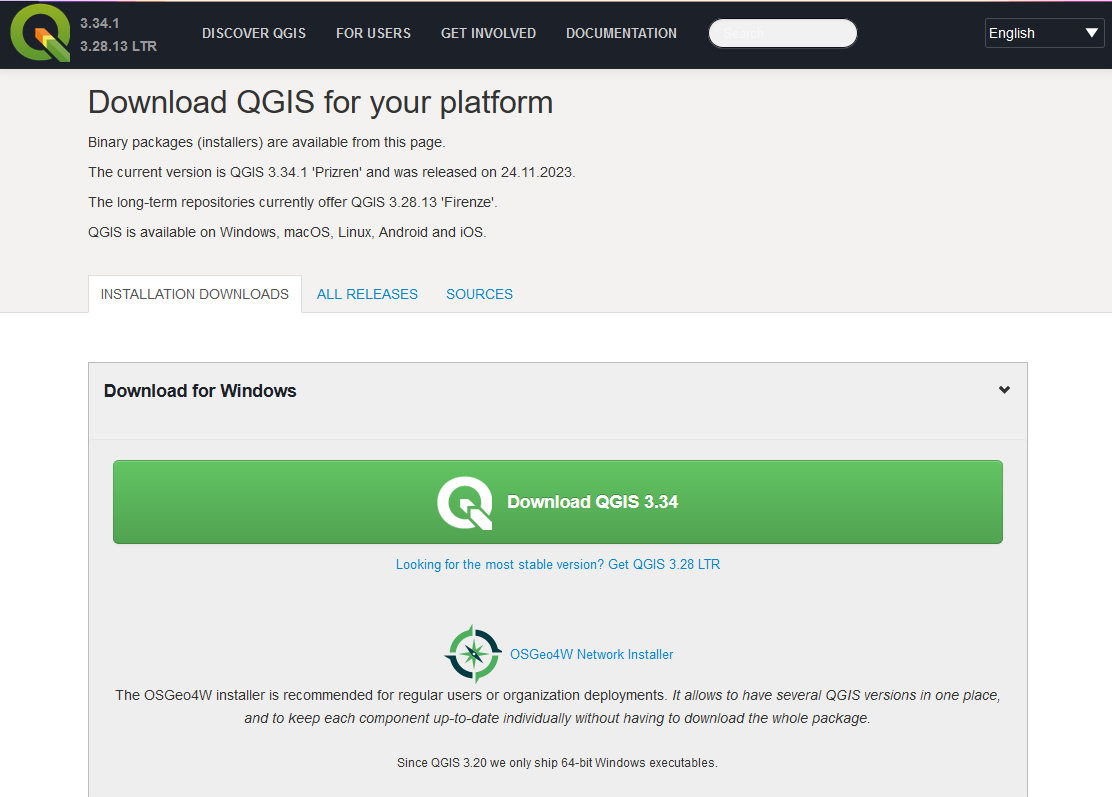
\includegraphics{./images/download_page.png}}

}

\caption{QGIS Download Page on Windows}

\end{figure}

Downloads of QGIS for Windows and MacOS, as well as instructions for
installing on other environments (linux, mobile) are available from the
\href{https://qgis.org/en/site/forusers/download.html}{downloads page of
the QGIS website}. When users go to the QGIS downloads page, they should
generally see the download options relevant to their operating system.
Windows and MacOS should be able to run the installer that downloads for
the selected version and be able to get going (but see any notes on the
download page); Linux users should review the instructions available for
their specific Linux distribution.

\hypertarget{available-versions}{%
\subsection{Available Versions}\label{available-versions}}

At the time of this writing, there are two versions of QGIS readily
available, and this general model is how it tends to be set up:

\begin{itemize}
\tightlist
\item
  Latest Release, version 3.34, available from the Green Button - this
  may have some newer features added;
\item
  Long Term Release (``LTR''), version 3.28, in the link directly below
  the green button - long term releases are maintained with bug-fixes,
  but not generally new features for 3 release cycles, to focus on
  stability.
\end{itemize}

This tutorial was developed using 3.34, but either version should
generally work. (Releases are denoted as x.y.z, where changes in `x'
denotes some potentially larger changes in the software, changes in `y'
denote additions of features and bug fixes, and changes in `z' generally
reflect bug-fixes.)

Should users need older or development releases for any reason, they can
access those through the ``All Releases'' tab on the webpage.

\emph{Note: Windows users will also notice another download option for
the OSGeo4W Installer, associated with a compass rose icon - this is an
installer that supports more customization of the installation -
advanced users may find this useful, for example to install development
versions of the software or specific versions of the libraries QGIS
depends on.}

\hypertarget{starting-qgis-and-installing-plugins}{%
\section{Starting QGIS and Installing
Plugins}\label{starting-qgis-and-installing-plugins}}

Once QGIS is installed, users should be able to go to their start menu,
desktop, or similar to find it and use the typical approach for starting
software on their operating system.

\hypertarget{plugins}{%
\subsection{Plugins}\label{plugins}}

As with many software packages, QGIS supports plugins - or basically
additional tools that can be written for the software to extend
functionality. There are hundreds of plugins available, all freely
available. To view and manage plugins, go to the \texttt{Plugins} menu
at the top and navigate to \texttt{Manage\ and\ install\ plugins}

\begin{figure}

{\centering 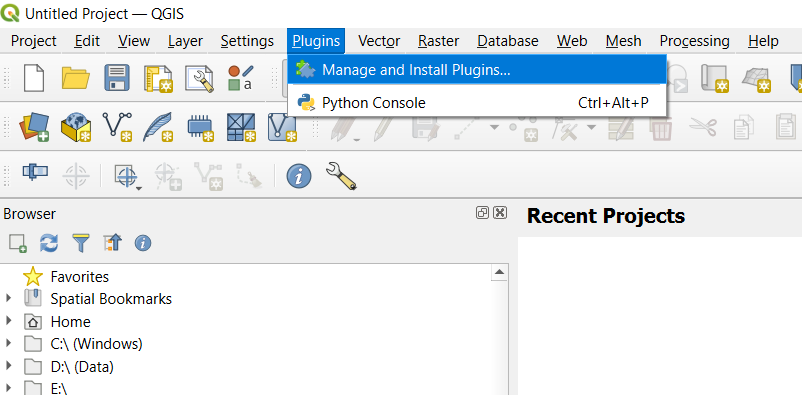
\includegraphics{./images/ToolbarToPlugins.png}

}

\caption{Getting to Plugins}

\end{figure}

The The following dialogue box will open, allowing users to browse
through or search available plugins, and then by using the tabs on the
left, seeing what plugins are installed and so-forth.

\begin{figure}

{\centering 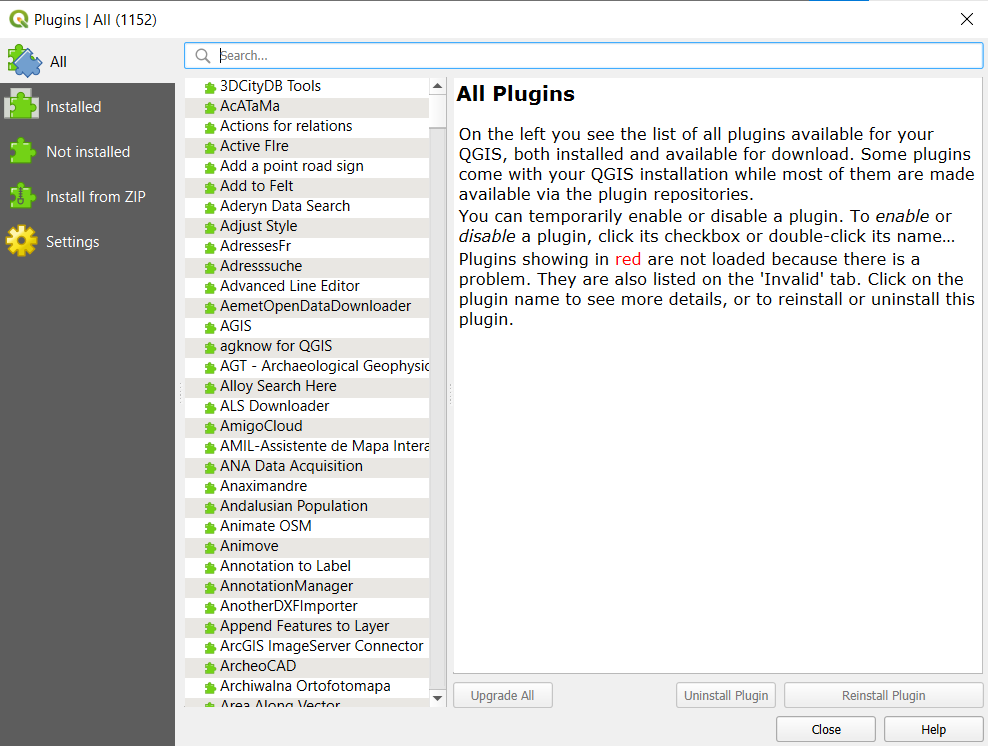
\includegraphics{./images/PluginsWindow.png}

}

\caption{Plugins Window}

\end{figure}

This tutorial makes use of the following plugins:

\begin{itemize}
\tightlist
\item
  Value Tool
\item
  QuickMapServices
\end{itemize}

To install the plugins, you can you can click the ``Install Plugin''
button that will appear when you select plugins from the list. Once
plugins are installed, you can use the checkboxes that appear alongside
those to enable or disable them; as plugins are installed, some may
result in a new window being shown automatically, or a new ``panel''
available from the \texttt{View} menu; some may result in new icons
appearing in the toolbar, a new menu being available at the top of the
QGIS window.

\hypertarget{basic-navigation-in-qgis}{%
\section{Basic Navigation in QGIS}\label{basic-navigation-in-qgis}}

When you open QGIS, you should see a window like the following.

\begin{figure}

{\centering 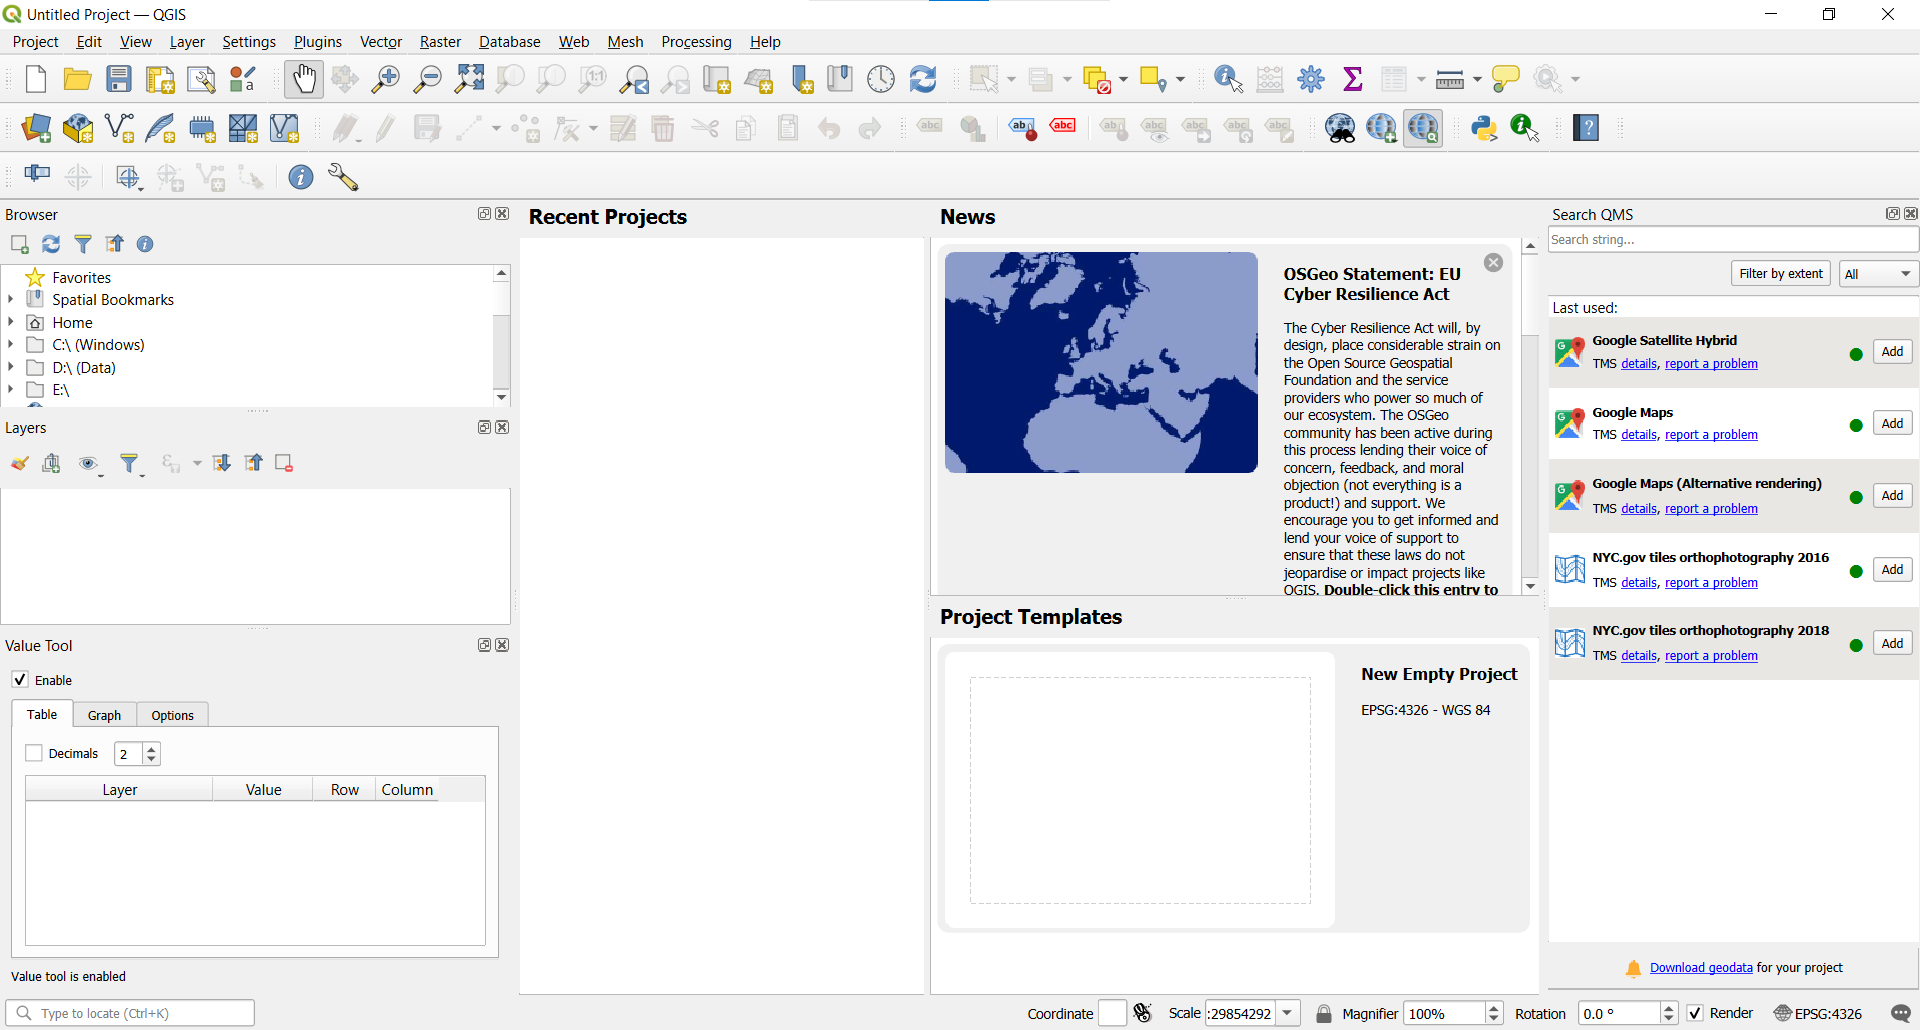
\includegraphics{./images/MainQGISWindow_PluginsInstalled.png}

}

\caption{First Look at the main QGIS Window (after Value Tool and
QuickMapServices plugins have been installed)}

\end{figure}

The labeled ``sub-windows'' you see, such as for the \emph{Browser},
\emph{Layers}, \emph{Value Tool} and so forth are referred to as panels
and the rows of icons across the top are toolbars. You can adjust what
you are seeing in terms of panels and toolbars by going to the
\texttt{View} menu a the top of the QGIS window, and selecting
\texttt{Panels} or \texttt{Toolbars} appropriately (right-clicking on
the toolbar also lets you see and turn on/off the panels and toolbars).
Some icons may seem fairly intuitive, such as to zoom in
(\includesvg{index_files/mediabag/mActionZoomIn.svg}) or zoom out
(\includesvg{index_files/mediabag/mActionZoomOut.svg}), but others may
not be, so explore and don't be afraid to try things out! It's generally
helpful to do this with smaller datasets loaded into QGIS to help
iterate through the different tools and options more quickly.

\textbf{\emph{I strongly encourage users to explore QGIS to familiarize
themselves a bit with the software - hover your mouse over icons to see
what they say, click on menu items at the top and browse around,
selecting through some different menus and such. QGIS is rich in
functionality, with multiple ways to do many things, so this can help
you figure out what the easiest ways are for you to approach
workflows.}}

\hypertarget{some-initial-setup}{%
\subsection{Some initial setup}\label{some-initial-setup}}

User may develop their own preferred ways of customizing things with any
software. Here are two initial things I like to do for QGIS:

\begin{itemize}
\tightlist
\item
  Delineate ``Favorites'' in the Browser panel:

  \begin{itemize}
  \tightlist
  \item
    The Browser panel is a bit of a ``one-stop-shop'' to navigate around
    your local file system and load various types of layers.
  \item
    If you navigate around the directories from within the Browser panel
    (expand what you see by clicking on the right-facing arrow to the
    left of a given name), you can right-click folders and select them
    as ``Favorites.'' If you keep files with data you use in some
    general locations, this can help save time to get to them -
    particularly if the data are several folders deep or something.
  \end{itemize}
\item
  Make the ``Processing Toolbox'' panel visible:

  \begin{itemize}
  \tightlist
  \item
    In QGIS, there are many tools accessible through the toolbars and
    menus at the top. The panel for the Processing Toolbox serves as a
    bit of a directory of all of the different tools that exist in QGIS.
  \item
    You can make this panel active either by going through the
    \texttt{View} menu -\textgreater{} \texttt{Panels}, or by clicking
    the \texttt{Processing} menu at the top and clicking on ``Processing
    Toolbox.''

    \begin{itemize}
    \tightlist
    \item
      The screenshot below shows what this looks like (with the
      Processing Toolbox panel active). The Processing Toolbox has been
      scrolled down to show \href{https://gdal.org/}{GDAL} and
      \href{https://grass.osgeo.org/}{GRASS} - these are two software
      packages installed with QGIS and accessible through the Processing
      Toolbox. (GDAL is the core software in QGIS generally underlying
      import/export operations, and with additional functionality
      available for various processing steps).
      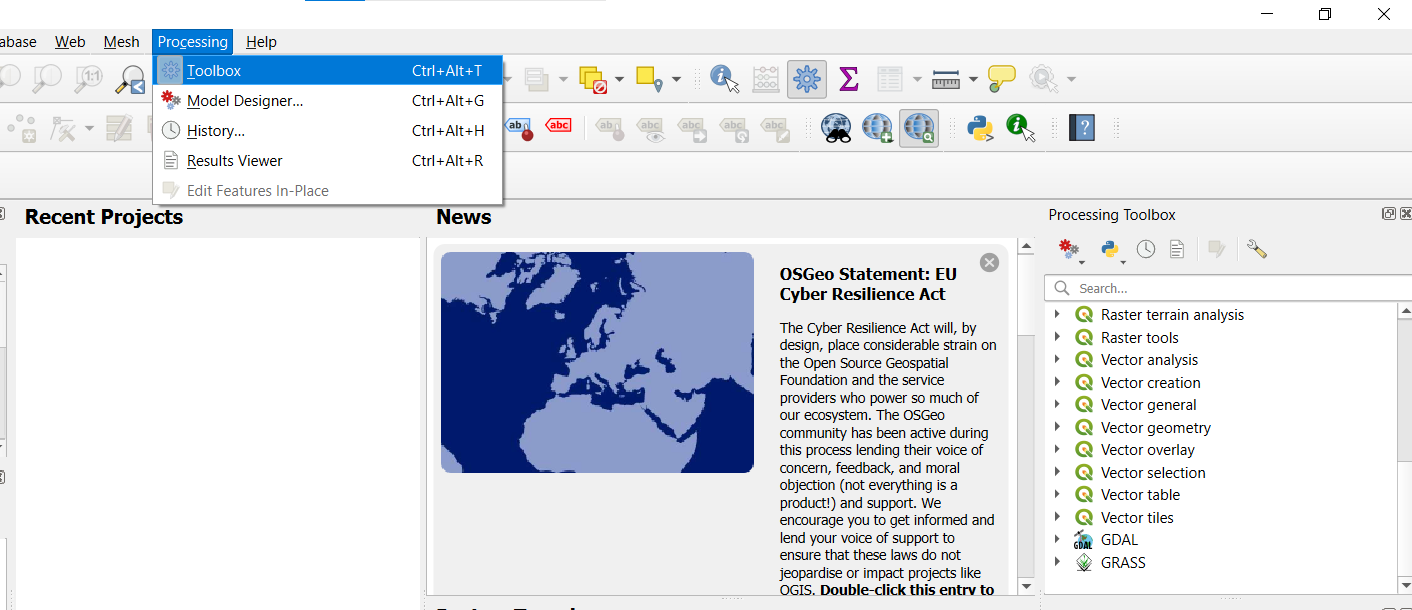
\includegraphics{./images/ProcessingToolbox.png}
    \end{itemize}
  \end{itemize}
\end{itemize}

Depending on what you are doing at a given time, you can ``x'' out of
individual panels and then re-instantiate them using \texttt{View}
-\textgreater{} \texttt{Panels} and you can resize them, pop them out,
etc. by clicking on the top of each panel (at about the same area where
the panel name is) and dragging it as desired.

\bookmarksetup{startatroot}

\hypertarget{tutorial-data}{%
\chapter{Tutorial Data}\label{tutorial-data}}

The data used in this tutorial are all freely available, at least under
creative commons licenses for non-commercial purposes, if not fully
public domain. These are all focused on New York City.

\textbf{\emph{\href{./QGIS_Tutorial_Data.zip}{Click Here to Download the
Tutorial Data}}}

\hypertarget{list-of-tutorial-data}{%
\section{List of Tutorial Data}\label{list-of-tutorial-data}}

The data are all made available in a .zip file associated with the
tutorial, and original sources are detailed below and each dataset is in
a folder with the respective \textbf{\emph{italicized \& bolded}} name
as follows, and the data files have their names in
\texttt{code-formatted\ text} (sometimes they are within their own
\texttt{.zip} files):

\begin{itemize}
\tightlist
\item
  \textbf{\emph{Vegetation Density Across NYC}} -
  \texttt{nyc\_propveg2017\_200mbuffer\_100ftgrid\_nowater.tif}:

  \begin{itemize}
  \tightlist
  \item
    a raster dataset where the value of each pixel represents the
    proportion of land cover within a 200 meter radius that was
    vegetated based on 6'' resolution land cover data for NYC
    representing 2017. Each pixel represents a 100 foot by 100 foot area
    on the ground. The data are available on a data repository,
    \href{https://zenodo.org/records/8370381}{Zenodo}.
  \end{itemize}
\item
  \textbf{\emph{Community District Boundaries}} - \texttt{nycd.shp}:

  \begin{itemize}
  \tightlist
  \item
    a vector dataset of (multi)polygons representing the 59 Community
    Districts in NYC, each of which has an associated Community Board
    \href{https://www.nyc.gov/site/planning/data-maps/open-data/districts-download-metadata.page}{NYC
    Department of City Planning Website}. The version available here was
    the version already clipped to shorelines, and associated with NYC
    Department of City Planning release ``23D.''

    \begin{itemize}
    \tightlist
    \item
      \emph{Note, this dataset is a shapefile, which involves not only
      the \texttt{.shp.} file but a number of other, ``sidecar'' files.
      For the shapefile to work correctly, all of the other associated
      files must be kept with it, in the same folder.}
    \end{itemize}
  \end{itemize}
\item
  \textbf{\emph{NYC Heat Vulnerability Index by Community District
  (2018)}} -
  \texttt{NYC\ EH\ Data\ Portal\ -\ Heat\ vulnerability\ index\ (full\ table).csv}:

  \begin{itemize}
  \tightlist
  \item
    The NYC Department of Health and Mental Hygiene produces the Heat
    Vulnerability Index (HVI) dataset to reflect the risk of
    community-level heat impacts, like deaths, due to extreme heat
    events; the index ranges 1-5, and higher numbers reflect higher
    vulnerability. The data used in this tutorial are based on a 2018
    version of the dataset; a newer version, recently released in 2023,
    is available from the
    \href{https://a816-dohbesp.nyc.gov/IndicatorPublic/data-explorer/weather-related-illness/?id=2191\#display=summary}{NYC
    Environment and Health Data Portal} but with some limits in ability
    to join to other data at this point.
  \end{itemize}
\item
  \textbf{\emph{Tree Canopy and Street Tree Summary Data}} -
  \texttt{canopy\_streettree\_supp.gpkg}:

  \begin{itemize}
  \tightlist
  \item
    This file includes data on tree canopy change (2010-2017) and street
    trees aggregated to political and administrative units of Boroughs,
    Community Districts, City Council Districts (2010), and Neighborhood
    Tabulation Areas (2010).
  \end{itemize}
\item
  \textbf{\emph{Green Roof Data (Centroids) for NYC}} -
  \texttt{GreenRoofData2016\_20180917.csv}:

  \begin{itemize}
  \tightlist
  \item
    Comma separated values file with the only spatial data for the green
    roofs being coordinates for the centroids in columns of
    \emph{xcoord} and \emph{ycoord}. The original dataset, along with
    more complete spatial data (green roof footprints) and full
    information about it is available on
    \href{https://zenodo.org/records/1469674}{Zenodo}.
  \end{itemize}
\item
  \textbf{\emph{NYS Disadvantaged Communities 2023}} -
  \texttt{Final\_DAC\_Attributes.shp}:

  \begin{itemize}
  \tightlist
  \item
    Shapefile with a dataset developed by the New York State Climate
    Justice Working Group, identifying areas with ``disadvantaged
    communities to ensure that frontline and otherwise underserved
    communities benefit from the state's historic transition to cleaner,
    greener sources of energy, reduced pollution and cleaner air, and
    economic opportunities.'' The data, based on Census Tract polygons,
    along with documentation and an interactive map is available from
    \href{https://climate.ny.gov/Resources/Disadvantaged-Communities-Criteria}{a
    New York State Government website}.

    \begin{itemize}
    \tightlist
    \item
      \emph{Note, this dataset is a shapefile, which involves not only
      the \texttt{.shp.} file but a number of other, ``sidecar'' files.
      For the shapefile to work correctly, all of the other associated
      files must be kept with it, in the same folder.}
    \end{itemize}
  \end{itemize}
\end{itemize}

\hypertarget{a-note-about-data-in-.zip-files-in-qgis}{%
\subsection{A note about data in .zip files in
QGIS}\label{a-note-about-data-in-.zip-files-in-qgis}}

In many cases, data are made available in a compressed, \texttt{.zip}
format - this tends to particularly hold true when multiple files are
shared together, either for functionality (e.g., with shapefiles and the
associated sidecar files), or to ensure metadata stays with the
associated data files. For many software packages, to even use the data
in these files, they need to be ``extracted'' from the \texttt{.zip}
format, and this functionality is generally included in a given
operating system, third party tools (e.g., free and open source
\href{https://www.7-zip.org/}{7-zip}). And for working with the
tutorial, it is recommended that you do unzip the main folder of data
made available.

However, it is possible to work with data in read-only mode (i.e., edits
to datasets downloaded cannot be made) - and this is often a good use
case for spatial data processing, in which edits files involves writing
out new data files. Thus, for working with the tutorial data, you can
opt to leave any data in \texttt{.zip} files as they are. If you find
that viewing or working with the data is slow, you may try unzipping the
files to see if it makes a difference, but some benefits I see of
working with the \texttt{.zip} files are:

\begin{itemize}
\tightlist
\item
  Keeping the ``raw'' or ``source'' data for a project uneditable in the
  \texttt{.zip} format helps ensure you can always go back to that
  original dataset if needed.
\item
  By not unzipping the data, you can reduce the storage space required
  for your project on your hard drive, since uncompressing may increase
  the size, and unless you delete the compressed files, there will be
  somewhat duplicate files on your drive. This can also help users keep
  data a bit better organized, simply because of the fewer folders and
  files.
\end{itemize}

This functionality in QGIS to work with uncompressed data (among other
things), made possible by the \href{https://gdal.org}{Geospatial Data
Abstraction Library (GDAL)}, in implementation of
\href{https://gdal.org/user/virtual_file_systems.html}{\emph{virtual
file systems}}.

\bookmarksetup{startatroot}

\hypertarget{loading-and-visualizing-data}{%
\chapter{Loading and Visualizing
Data}\label{loading-and-visualizing-data}}

\hypertarget{importing-data-already-in-gis-formats}{%
\section{Importing Data Already in GIS
Formats}\label{importing-data-already-in-gis-formats}}

There are a few different workflows that can be used to bring data into
QGIS. Thankfully, for data already in GIS formats (e.g., shapefiles,
geopackages, filegeodatabases, geotiffs), the steps can be as simple as
\textbf{drag and drop the file from your file explorer (e.g., Windows
Explorer on Windows) into the QGIS Window}. This generally involves
having your file explorer open in the foreground over QGIS, and then
clicking and holding on the desired file, and dragging it into the QGIS
window, and releasing the click.

\begin{figure}

{\centering 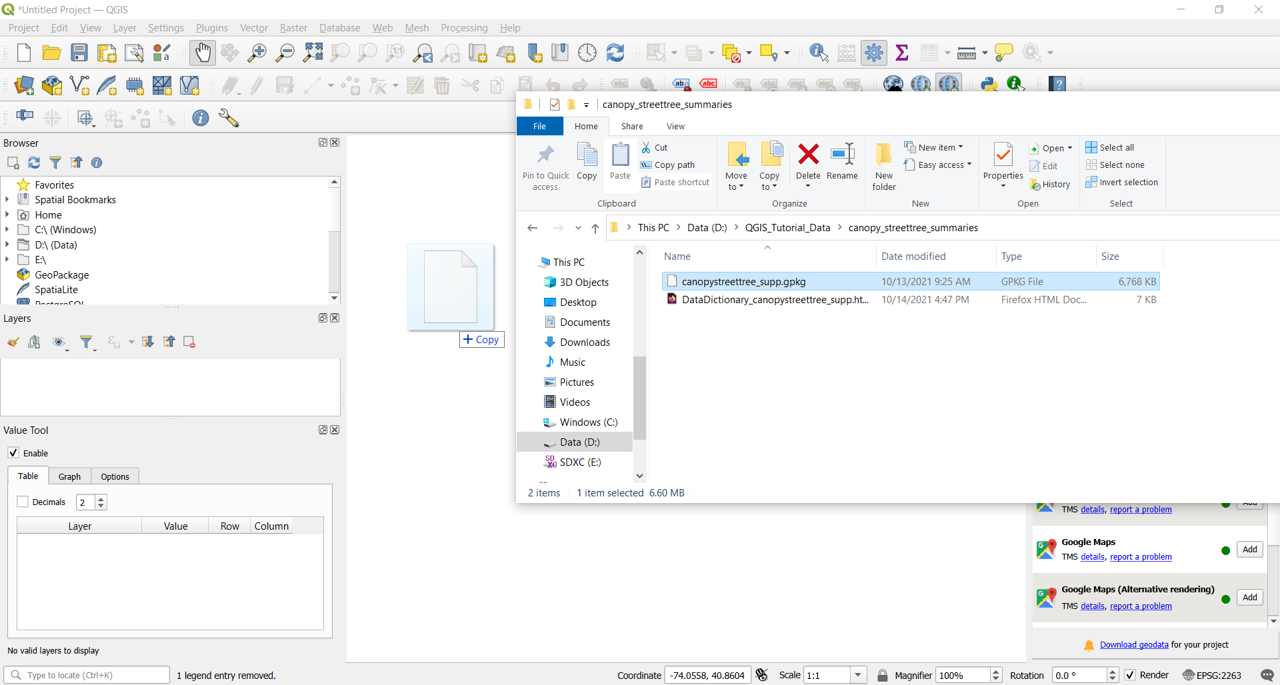
\includegraphics{./images/draganddrop_data.png}

}

\caption{Example of loading data into QGIS by dragging and dropping a
file}

\end{figure}

\textbf{Try this with the Tree Canopy and Street Tree Summary Data,
\texttt{canopystreettree\_supp.gpkg} - just load the layer named
\emph{canopystreettree\_supp\_communitydist} for now}

Similarly, users can navigate to location of desired files in the
Browser panel and drag the files into the Layers panel or the main
panels toward the middle of the QGIS window.

*** Note - when you first load a vector dataset, the symbology will
typically be the same for the entire layer and the color of the symbols
will be randomly generated.***

Some data formats, such as geopackage (\texttt{.gpkg}) and Esri file
geodatabases (\texttt{.gdb}) can contain multiple datasets (spatial and
non-spatial). When you go to load such data, where multiple datasets or
layers are included through one of these drag and drop approaches, you
will be prompted to select which data layers you want to include. The
default is they are all included. Additionally, by expanding the
\emph{Options} at the bottom, you can choose to import the selected
layers directly into a group, such that they are nested together in the
Layers panel.

\begin{figure}

{\centering 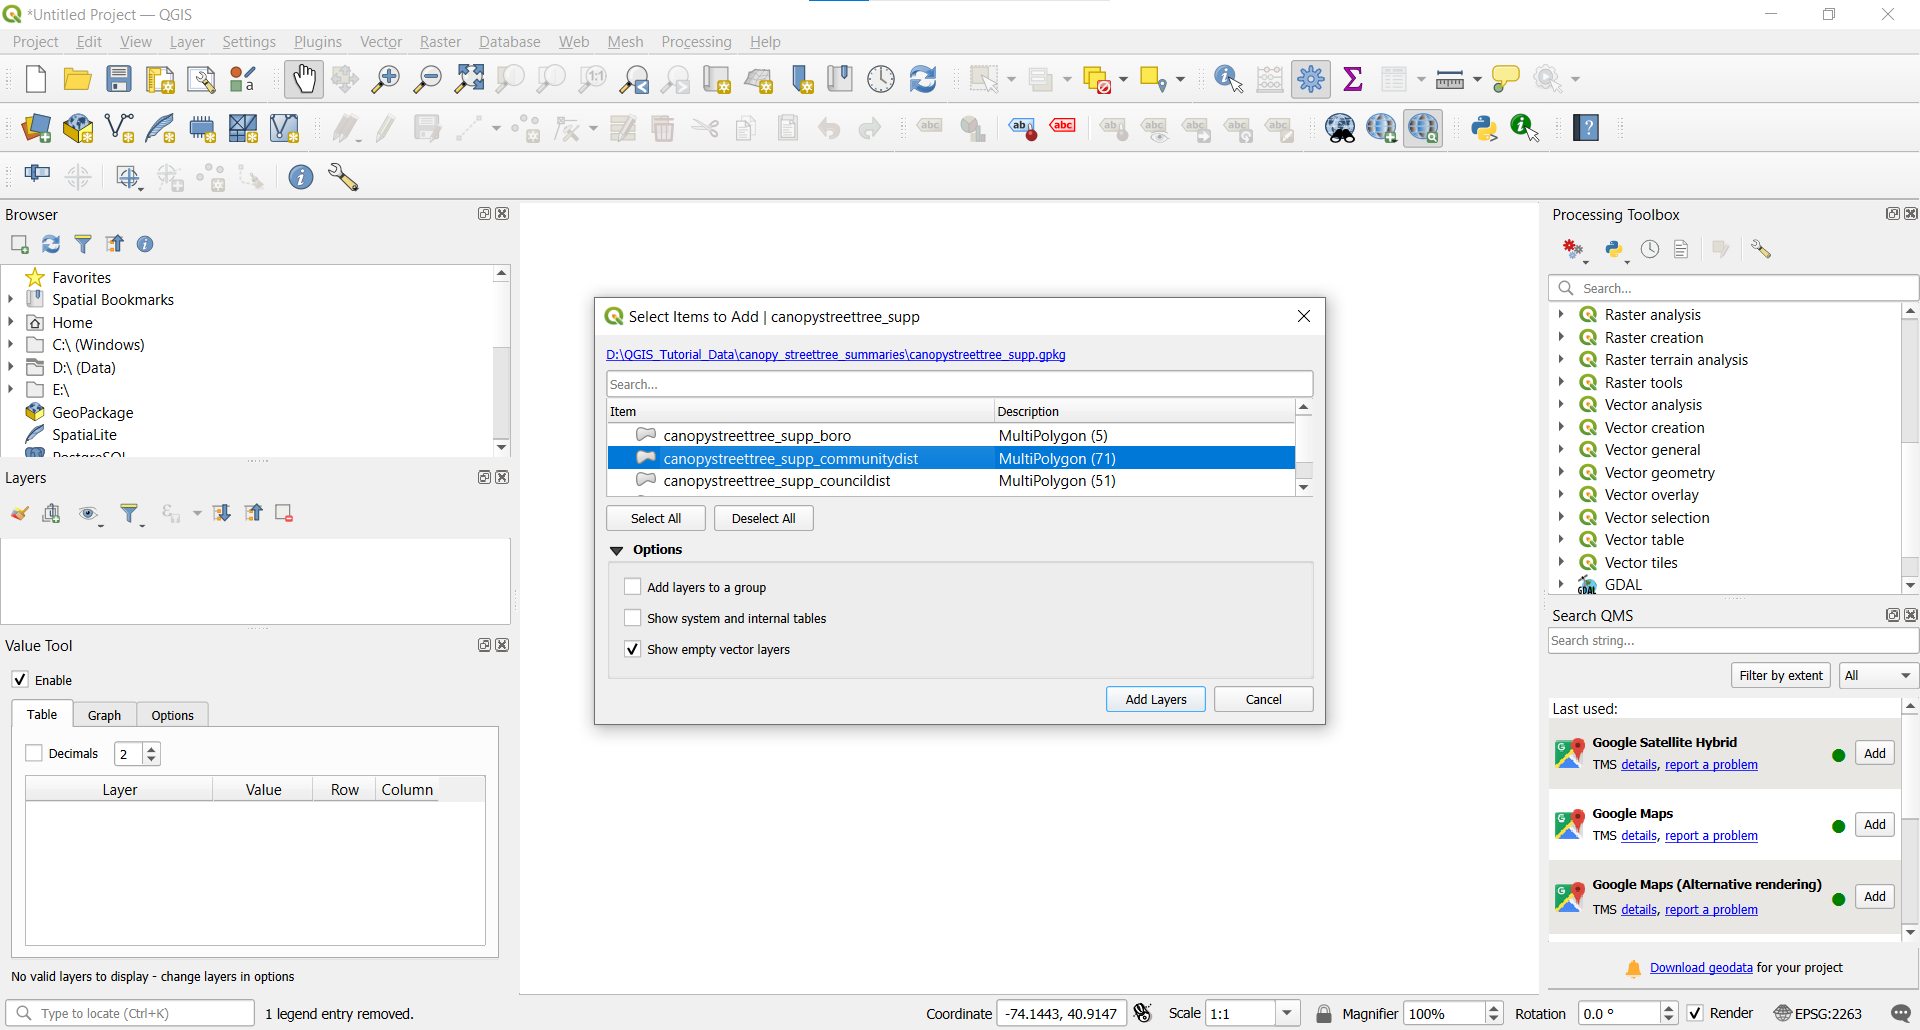
\includegraphics{./images/multi_table_import.png}

}

\caption{Example of loading multi-layer file into QGIS}

\end{figure}

Any tables of data in spatial formats without actual spatial data (e.g.,
non-spatial tables in a geopackage or file geodatabase) will simply
appear as a table in QGIS. The same is the case for any data in
non-spatial formats (e.g., text- or tab-delimited files).

\hypertarget{importing-data-in-delimited-text-e.g.-csv-files}{%
\section{Importing Data in Delimited Text (e.g., CSV)
Files}\label{importing-data-in-delimited-text-e.g.-csv-files}}

In many cases data are found in non-GIS data formats, such as
\texttt{.csv} files, which can be read into spreadsheet software such as
Excel. Spatial data in these files may be in the form of columns
representing x and y coordinates (for points) or in a single column with
the information stored in a ``WKT'' or ``Well-Known Text'' format, which
follows a specific convention for spatial information (this can include
data for (multi) points, lines, and polygons data).

The process for importing these datasets is inherently not as simple as
drag-and-drop, due to the fact that these files do not contain all of
the information GIS software would need to display them correctly - some
of it must be provided (or confirmed) by the user.

As an example, the data associated with this tutorial include a CSV file
with centroids of green roofs in NYC. One workflow for bringing this
dataset into QGIS is as follows:

\begin{itemize}
\tightlist
\item
  Open the \textbf{\emph{Data Source Manager}}
  (\includesvg{index_files/mediabag/mActionDataSourceMan.svg} -
  generally near the upper left in the toolbar; it is also available
  through CTRL+L on Windows and the \texttt{Layers} menu)
\item
  Select the \emph{Delimited Text} option on the left, use the
  ``\ldots{}'' to the right of the File name box box at the top to
  navigate to the file.

  \begin{itemize}
  \tightlist
  \item
    In this case, QGIS should automatically identify that it is a CSV
    file, and that the data are point coordinates, with the x- and
    y-fields being stored in the data in columns \emph{xcoord} and
    \emph{ycoord}, respectively. Users should always confirm QGIS is
    identifying such information correct.
  \item
    QGIS does not know what the CRS, or Coordinate Reference System is
    for these data, so the ``Geometry CRS'' entry says may either make
    an assumption, that it is in the same CRS as other data brought into
    QGIS already, or it will indicate ``invalid projection'' and this
    needs to be specified by the user.
    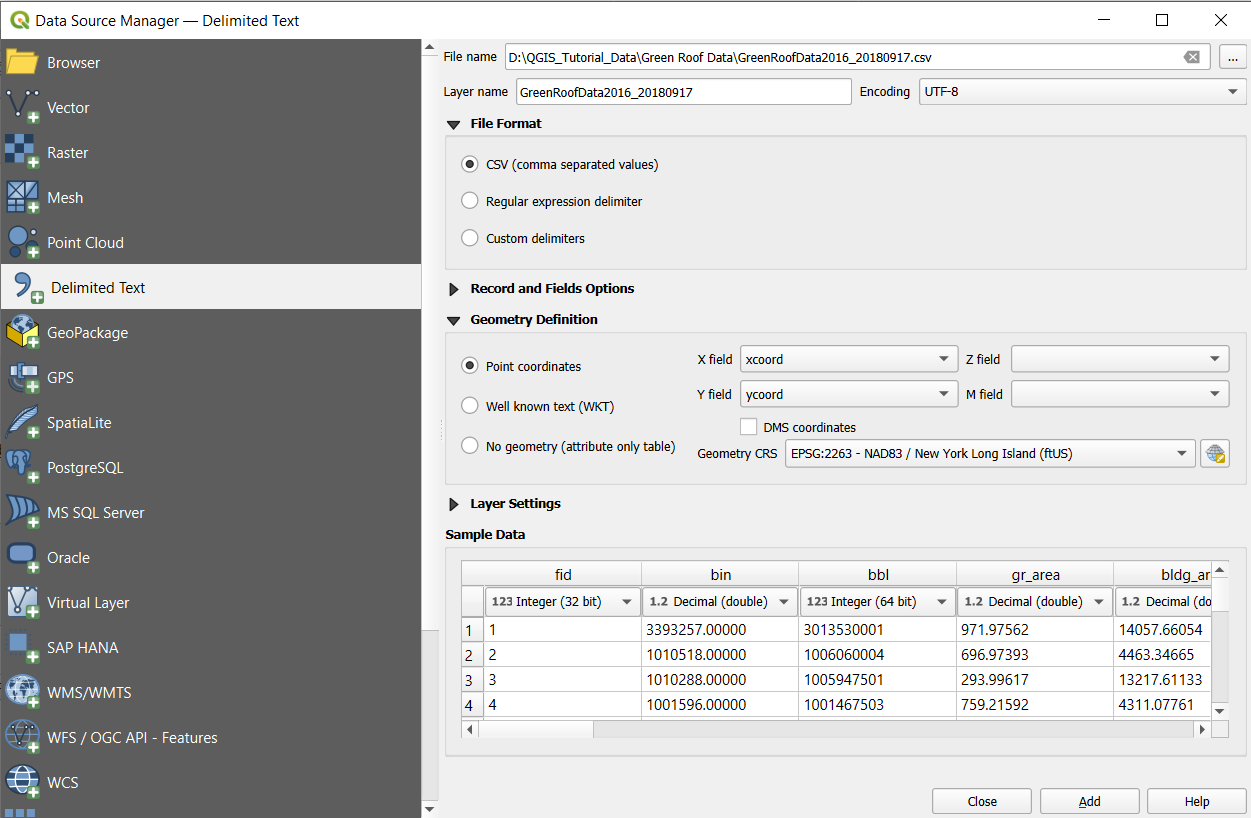
\includegraphics{./images/Load_CSV_PointData.png}

    \begin{itemize}
    \tightlist
    \item
      In either case for this dataset, you will need to indicate to QGIS
      the correct CRS. The previous dataset we have brought in by this
      point was in the \href{https://epsg.io/2263}{New York State Plane
      Long Island Zone, North American Datum of 1983, EPSG 2263}, in US
      Feet. However, this dataset has the coordinates in
      \href{https://epsg.io/4326}{Latitude/Longitude, in the WGS 84
      Datum, EPSG 4326}. Click on the icon to the right of this box
      about Coordinate Systems
      \includesvg{index_files/mediabag/mActionSetProjection.svg}
    \end{itemize}
  \item
    Then in the window that appears, use the text filter to search for
    `4326' - which is a shorthand reference, an ``EPSG'' code to the
    appropriate Coordinate Reference System these coordinates are in -
    (More about Coordinate Reference Systems in the next chapter,
    \protect\hyperlink{projections}{Coordinate Reference Systems}.)
    Expand the content in the next box, to reflect what you see in the
    screenshot below, and hit the Okay button.
    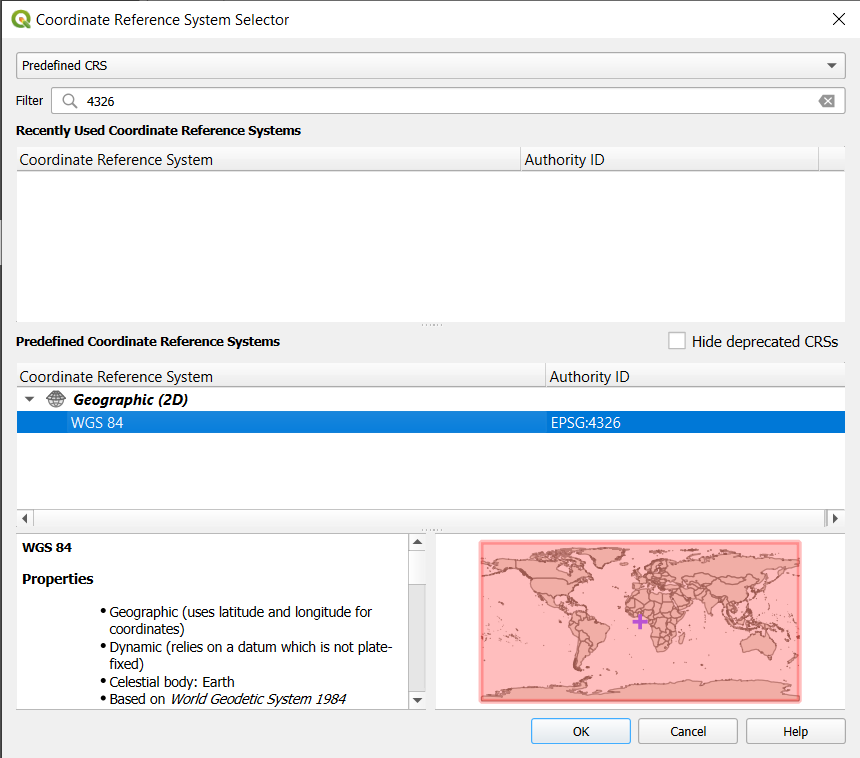
\includegraphics{./images/defining_crs.png}
  \item
    In the Data Source Manager, you should now be able to click the
    ``Add'' button (which would have been grayed out until the CRS is
    defined).

    \begin{itemize}
    \tightlist
    \item
      Before the dataset appears in the Layers panel, and the points
      appear in the main window of QGIS, you may see a window pop up
      asking you to select the desired operations to convert between
      coordinate systems. You can simply go with the default option and
      click ``OK.''
    \end{itemize}
  \end{itemize}
\item
  The data layer, layered on top of the other dataset we have brought in
  at this point should now appear something like the below (you'll need
  to close out the Data Source Manager window).
  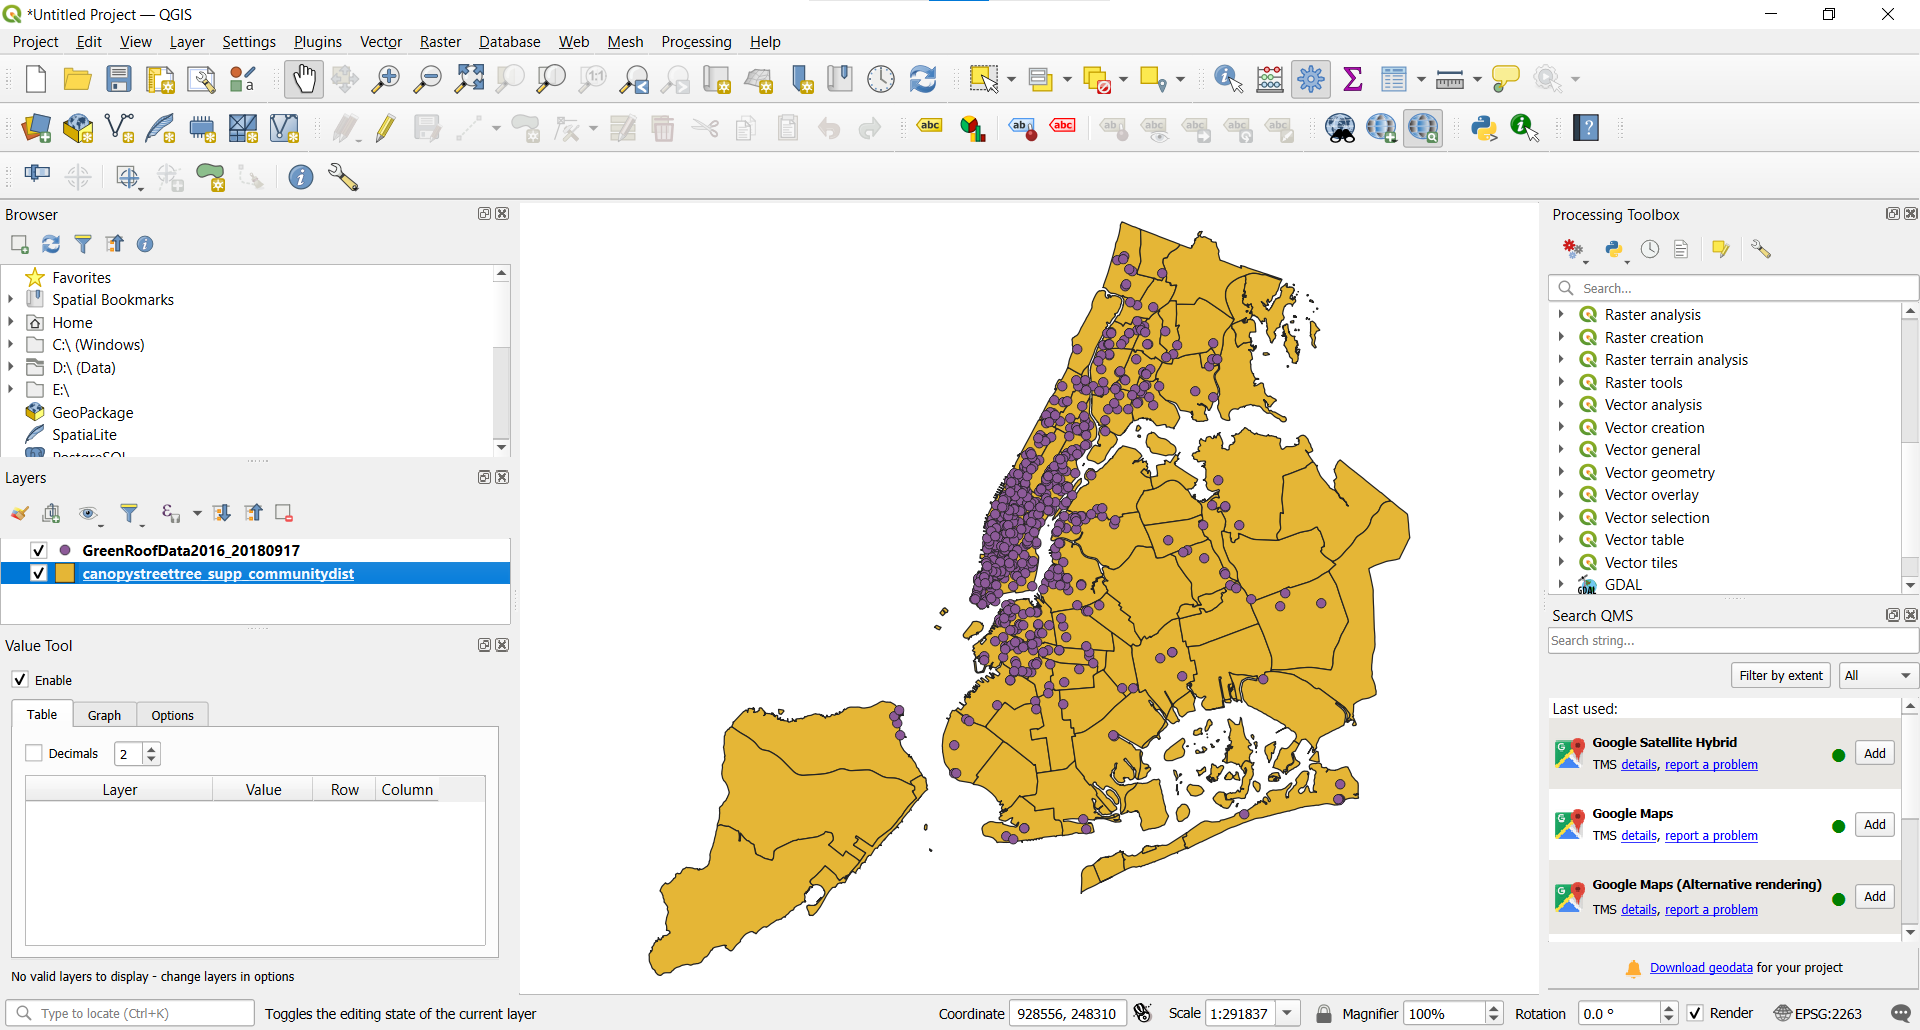
\includegraphics{./images/greenroofs_firstload.png}
\end{itemize}

** At this point, load in each of the other data layers (except for
other layers available with the Tree Canopy and Street Tree Summary data
- for that, the Community District layer is the only one you'll need).
For the remaining datasets you can drag and drop from your file explorer
or by navigating to them in the Browser panel; if the data are in
\texttt{.zip} folders, you can use those. \textbf{The NYC Heat
Vulnerability Index data is a tabular data, and will not show anything
in the main QGIS window, but we will use it later on.* }

\hypertarget{ordering-and-grouping-layers}{%
\subsection{Ordering and Grouping
Layers}\label{ordering-and-grouping-layers}}

As the data layers were loaded, they generally should be listed in the
Layers panel, in the order in which they were loaded (last layer at the
bottom). This also reflects the ordering in the main map area, or the
\emph{canvas} - with the layers higher in the list being ``on top''
visually (i.e., the dataset of green roof points should be visible on
top of everything else and you may not see some layers that are hidden
behind or below others).

To change which layers are visible, you can use the check-boxes, to make
them appear or disappear in the map canvas, and you can re-order in the
Layers panel by clicking and holding on the desired layer, and moving it
up or down with respect to the other layers.

Sometimes it is helpful to ``group'' layers - which has them nested
under a title within the Layers panel, and then they, as a group, appear
above or below the other layers based on the ordering within the panel.
There will also be a check-box next to the group label, which you can
use to turn on or off those layers together. To group/ungroup, select
the desired layers by using \texttt{CTRL\ +\ Click} on each layer (or
\texttt{SHIFT\ +\ Click} on the first and last layer if all
consecutively ordered), right click, and select ``Group Selected.''

\begin{figure}

{\centering 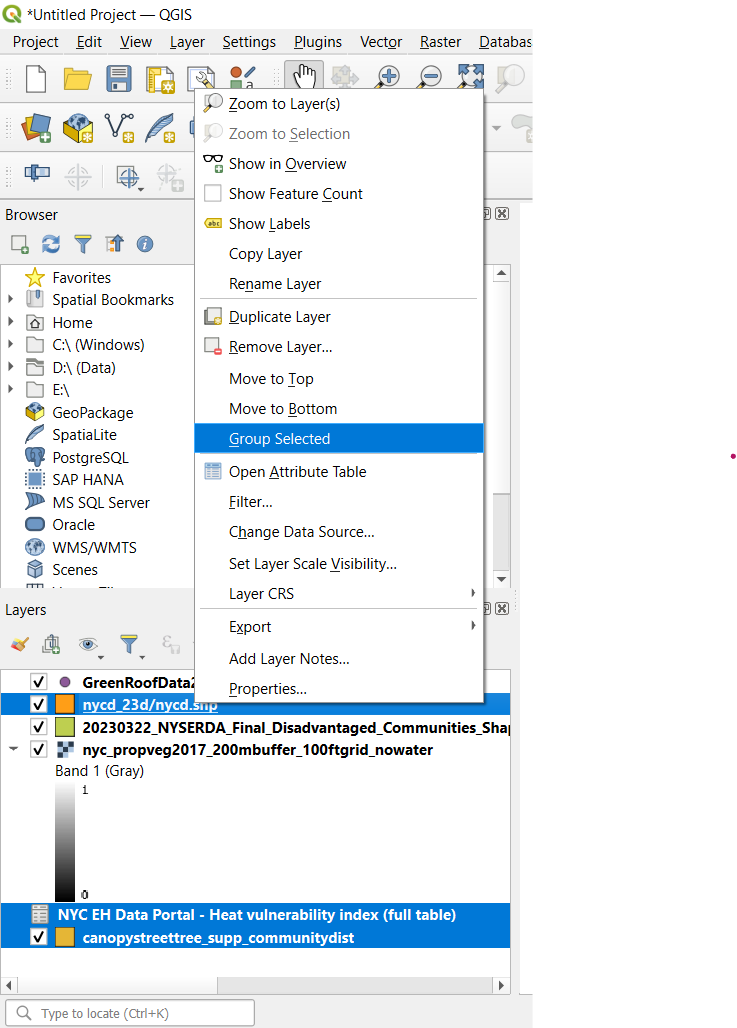
\includegraphics{./images/grouping.png}

}

\caption{Grouping layers by selecting the desired layers in the Layers
panel and right-clicking}

\end{figure}

You can then move layers into and out of the group by clicking/dragging
them around. You can also create a new group using the respective icon
at the top of the Layers panel
\includesvg{index_files/mediabag/mActionAddGroup.svg} and then drag
layers in and out as desired.

\begin{figure}

{\centering 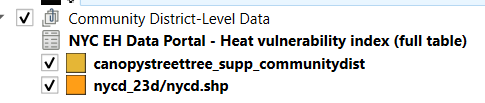
\includegraphics{./images/grouped_layers.png}

}

\caption{Example of grouped layers in the Layers panel}

\end{figure}

Upon creating a group, you can rename it by right clicking on it and
selecting ``Rename Group.'' Similarly, you can rename layers for use in
the QGIS project by right clicking on them and selecting ``Rename
Layer.''

\hypertarget{saving-a-project}{%
\subsection{Saving a Project}\label{saving-a-project}}

At this point, we've done a few different steps, and as with so much
work, would not want to have to redo things we've already done if
anything happens - the computer or software crashes. To do this the
first time, you can click the
\includesvg{index_files/mediabag/mActionFileSave.svg} on the toolbar,
navigate to the desired folder where you want to save the project, set a
name, and click ``Save.''

The default format is a \texttt{.qgz} file, which is suitable for most
use cases. If you are working on a shared drive with others, you may opt
to use the \texttt{.qgs} format, which at least in my experience, works
better if multiple people may be opening the project from different user
accounts (e.g., on a server).

As you work, you can click the
\includesvg{index_files/mediabag/mActionFileSave.svg} or use
\texttt{CTRL\ +\ S} on the keyboard to save as you go.

You can also save an existing project into a new file by using the
\texttt{Project} menu and selecting ``Save As'' or using
\texttt{CTRL\ +\ SHIFT\ +\ S} on the keyboard.

\hypertarget{viewing-attribute-information-for-layers}{%
\section{Viewing Attribute Information for
Layers}\label{viewing-attribute-information-for-layers}}

\hypertarget{attribute-tables}{%
\subsection{Attribute Tables}\label{attribute-tables}}

Data tables associated with vector datasets, and non-spatial tabular
data can be viewed in QGIS by right-clicking on the layer and selecting
``Open Attribute Table.'' For large datasets, it will take some time to
render, but generally for all of the datasets in this tutorial the
attribute tables should appear fairly quickly. In some cases you may
only want the attribute table to show a subset of the data, such as
those visible in the map canvas, and you can set this using the dropdown
menu at the bottom-left of the attribute table.

\begin{figure}

{\centering 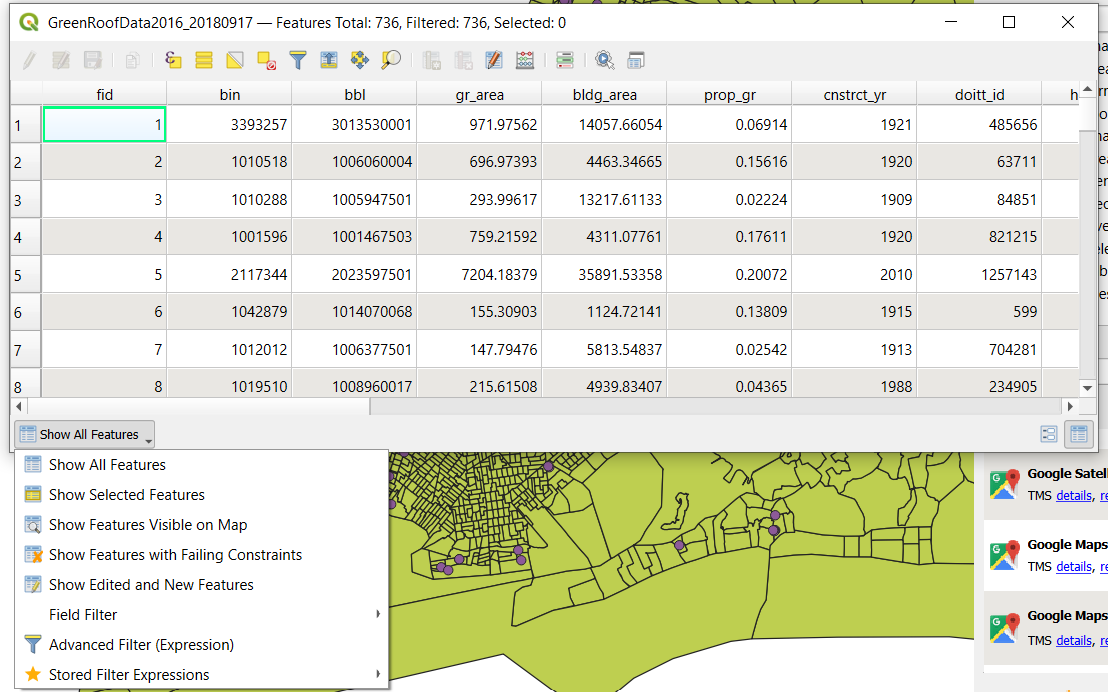
\includegraphics{./images/attribute_table_show_desired_features.png}

}

\caption{Attribute table for green roofs data shown, with the dropdown
menu expanded for limiting what is shown in the attribute table}

\end{figure}

\hypertarget{identify-features}{%
\subsection{Identify Features}\label{identify-features}}

To find out the attribute information for a given piece of a given
dataset, you can use the Identify Features tool from the toolbar
\includesvg{index_files/mediabag/mActionIdentify.svg}. Once selected,
you can either click on anything you see within a layer that is selected
(e.g., appears in gray) in the Layers panel, or you can right-click in
the map canvas and select the layer you want the information from. Once
you select the item the \textbf{Identify Results panel} will appear with
the respective information as shown below.

\begin{figure}

{\centering 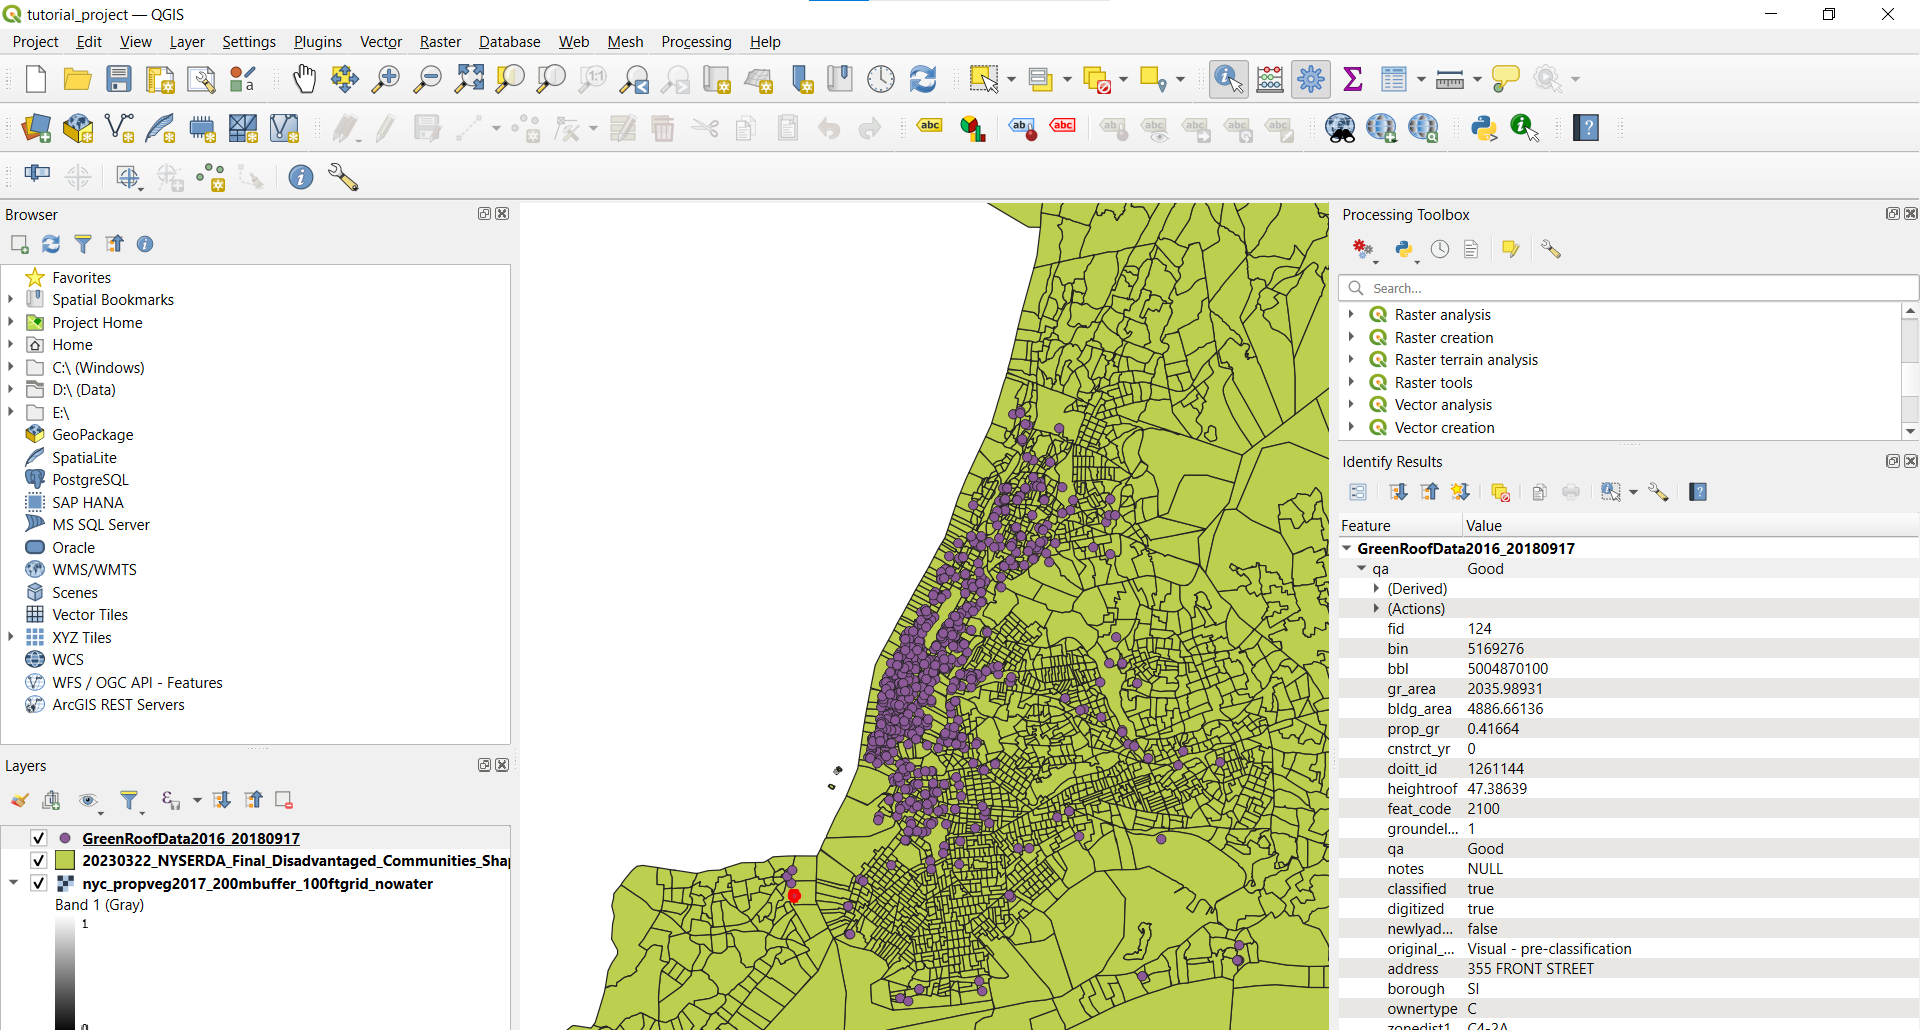
\includegraphics{./images/IdentifyFeatures.png}

}

\caption{Identify Features panel with information for the green roof
point, highlighted in red in the map canvas}

\end{figure}

If you are zoomed out enough such that you select multiple features, you
will be able to scroll down in the Identify Features panel and see the
different entries available. You can also adjust some options for the
Identify Features tool via the icons at the top of the panel.

\hypertarget{value-tool-for-raster-data}{%
\subsection{Value Tool (for Raster
Data)}\label{value-tool-for-raster-data}}

While the Identify Features tool works for raster data, as well as
vector data, the \emph{Value Tool plugin} can make for somewhat easier
inspection of raster data. With the \textbf{Value Tool panel} active
(click the \includesvg{index_files/mediabag/icon.svg}), as you move your
mouse across the canvas, it will show the values for the pixels from a
raster dataset (you may need to resize the columns to see the values).
The image below shows an example with the raster data from this
tutorial, with the ``Decimals'' box checked to only show two decimal
places of information in the Value column.

\begin{figure}

{\centering 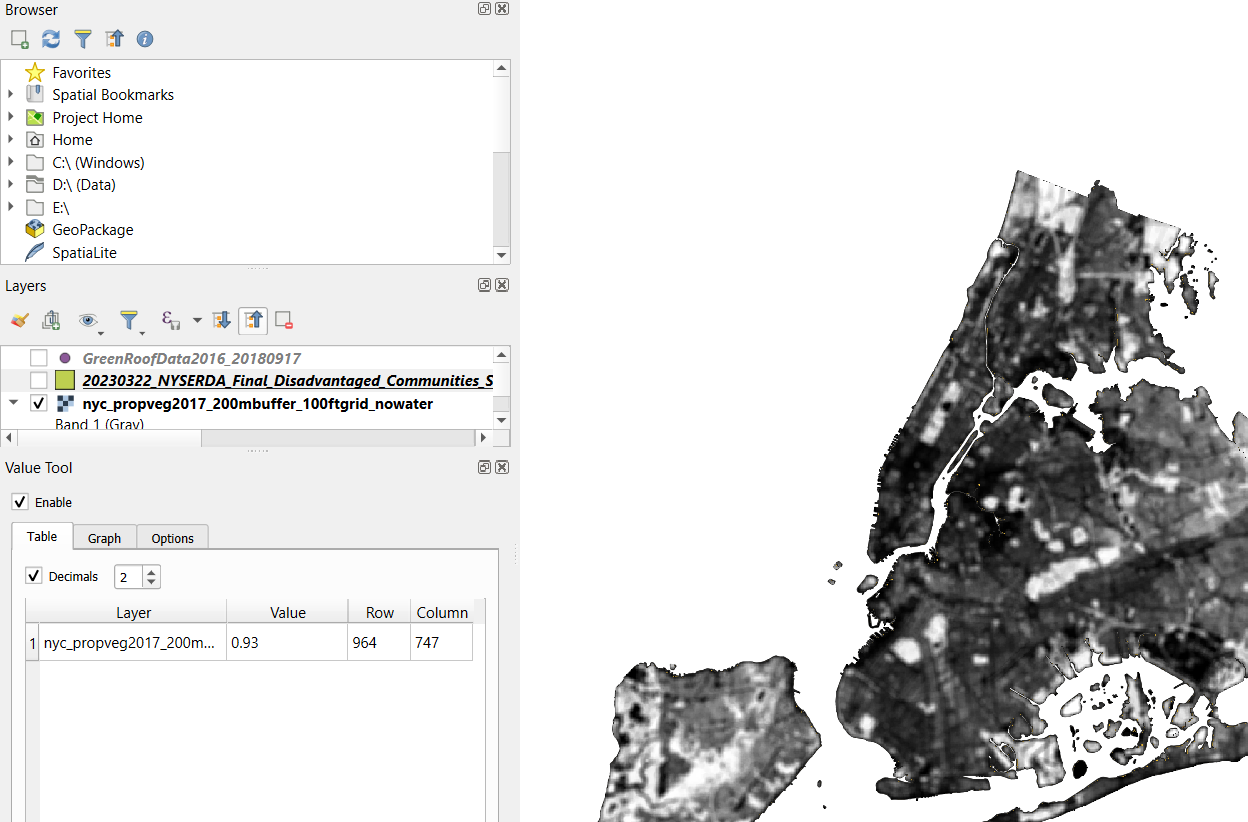
\includegraphics{./images/ValueToolExample.png}

}

\caption{Example of the Value Tool}

\end{figure}

As you mouse over the raster you will see the values change.

\hypertarget{basic-styling}{%
\section{Basic Styling}\label{basic-styling}}

As you look at data with different kinds of information, you likely want
to style it to your liking - either for making maps, or just getting
some specific insights. To get to the style settings, you can either
open the \textbf{Layer Styling panel} and select the desired layer in
the Layers panel, or you can right click/double clock on any layer in
the Layers panel, select ``Properties'' get to the \textbf{Properties
window} and click on the relevant tabs on the left to get to styling
menus for things like \emph{Symbology} \emph{Labels}. Users may find one
or the other approach works better for them. Due to the different nature
of vector and raster datasets, the styling menus are a bit different
across these two

\hypertarget{vector-styling}{%
\subsection{Vector Styling}\label{vector-styling}}

For vector data, the symbology options generally look along the lines of
the below (for the Green Roof Centroids dataset).

\begin{figure}

{\centering 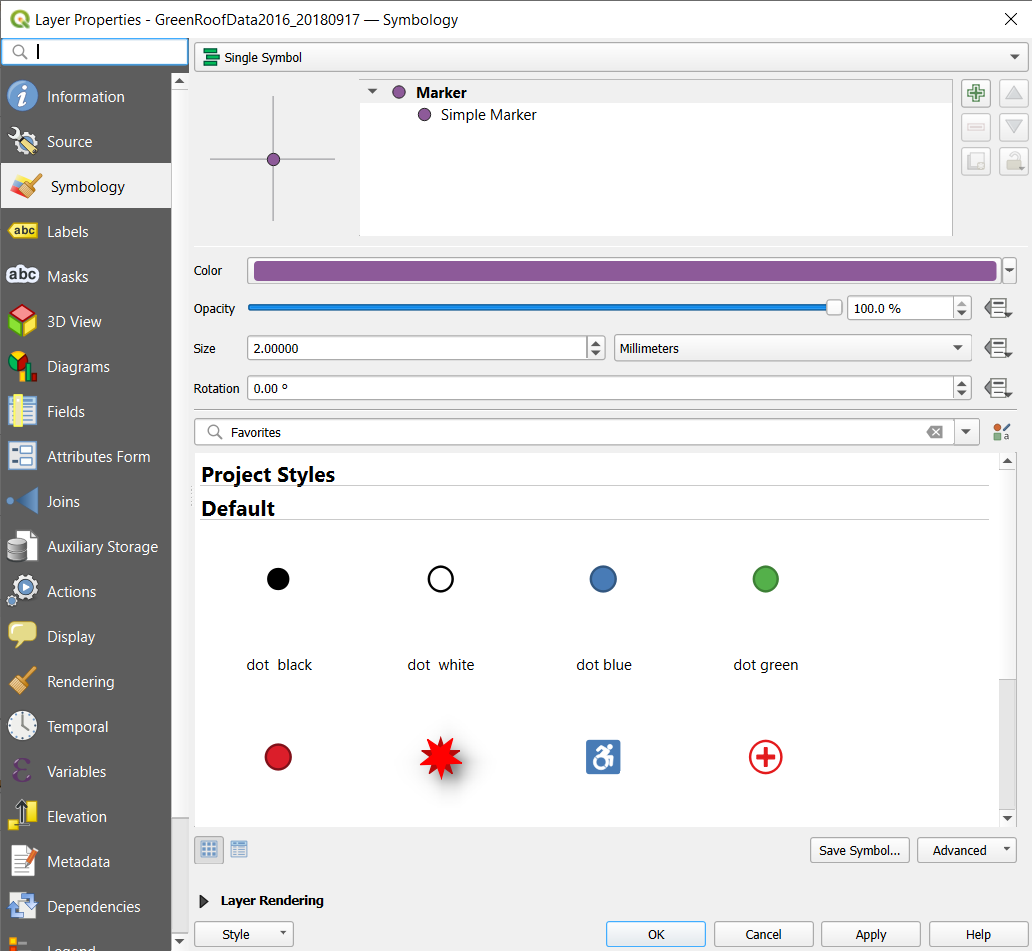
\includegraphics{./images/point_symbology_1.png}

}

\caption{Symbology menu for a point layer (the Green Roof Centroids
dataset in the Layer Properties Window}

\end{figure}

Users can do a variety of things here such as:

\begin{itemize}
\tightlist
\item
  Click in the colored box or use the dropdown icon to the right of it
  to select a different color, adjust some different parameters (e.g.,
  size and opacity);
\item
  Select a different initial symbol type from the set towards the bottom
  of the window;
\item
  Use the dropdown next to the word ``Favorites'' to access some
  different sets of symbol options or select the ``All Symbols'' option;
\item
  In the upper area, click on ``Simple Marker'' and adjust the various
  options that become visible;
\item
  Click the \includesvg{index_files/mediabag/mActionAdd.svg} towards the
  top to add multiple symbology types (e.g., for point data a second
  symbol could be added to be a bigger circle around the point);
\item
  Use the dropdown menu from the top for options to color different
  features in a relatively automated way.
\end{itemize}

There is \textbf{A LOT} to explore in terms of symbology. The
Categorized or Graduated symbology options from the dropdown menu at the
top is one of the most useful features in my work. As an example, with
the Green Roof Centroids dataset, if I choose the ``Graduated''
symbology option, I can than select for the ``Value'' field any numeric
variable; for this tutorial I'll chose \texttt{gr\_area} representing
the area of the green roof surface in square feet. Leaving Symbol type
as-is, I select a color ramp of Greens (light to dark greens), then
leave the ``Mode'' for the styling as ``Equal Count'' (which results in
about the same number of data points with each color along the gradient)
and hit ``Classify.''

\begin{figure}

{\centering 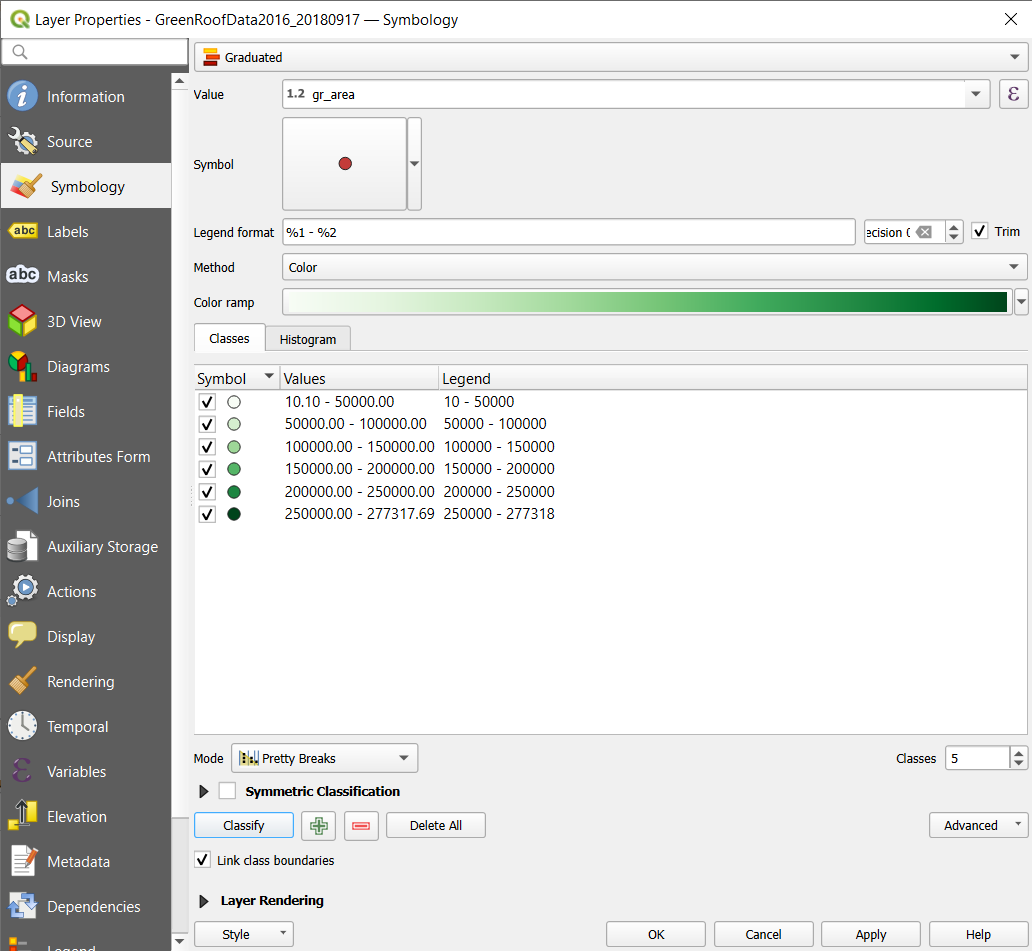
\includegraphics{./images/point_symbology_2.png}

}

\caption{Example of Layer Properties - Symbology menu for the Green Roof
Centroids Dataset, using a graduated symbology}

\end{figure}

After adjusting the settings, clicking ``OK'' will apply the styling
choices and close the window; clicking ``Apply'' will apply the styling
choices but leave the window open for further adjustments.

\begin{figure}

{\centering 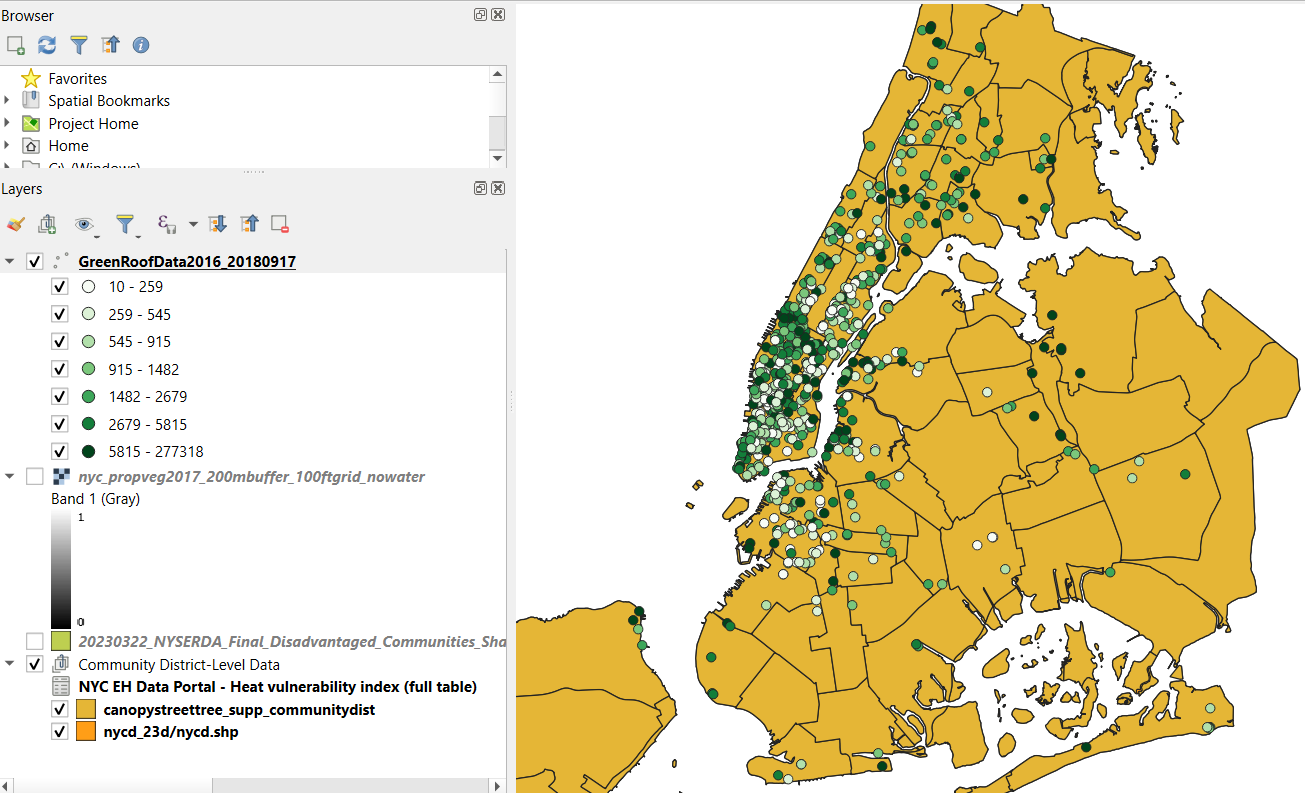
\includegraphics{./images/point_symbology_3.png}

}

\caption{The Green Roof Centroids dataset with a graduated style
applied}

\end{figure}

One thing that is sometimes useful is \textbf{having the border of
symbols be the same color as the symbols themselves}, and while one
could go symbol by symbol along a set of specific styles, some built-in
functionality makes this pretty easy in QGIS:

\begin{itemize}
\tightlist
\item
  In the main \emph{Layer Properties - Symbology} menu, select the
  Simple Marker (for a Single Symbol styles) or click on the default
  symbol for a Graduated, Categorized, or similar style and then to the
  Simple Marker
\item
  Click on the dropdown menu to the right of the ``Stroke Color'' then
  click ``Edit'' 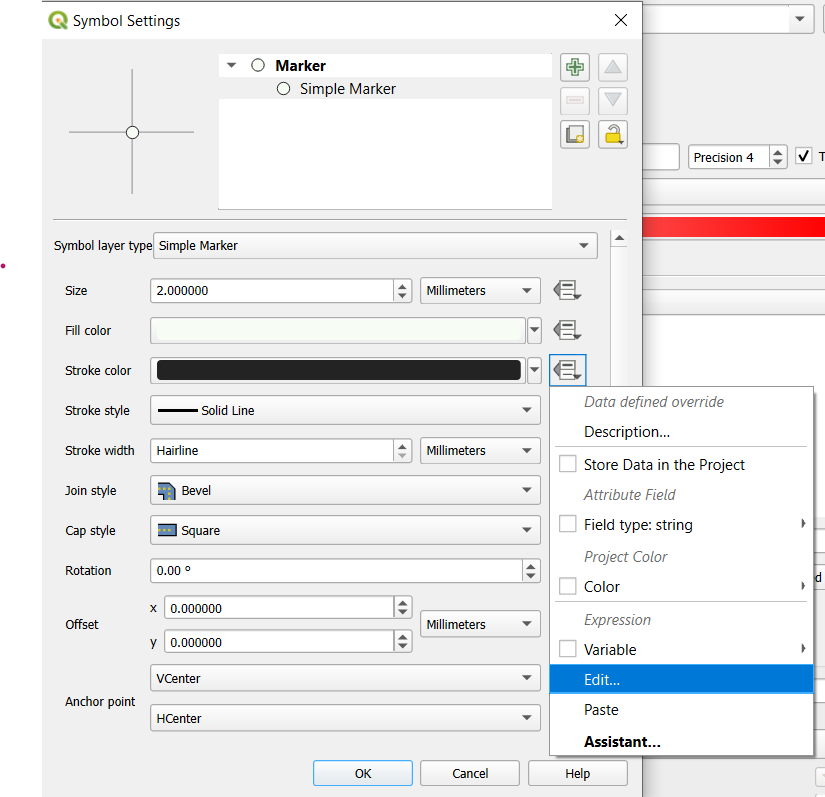
\includegraphics{./images/stroke_color_edit.png}
\item
  In in the box on the left type \texttt{@symbol\_color}
  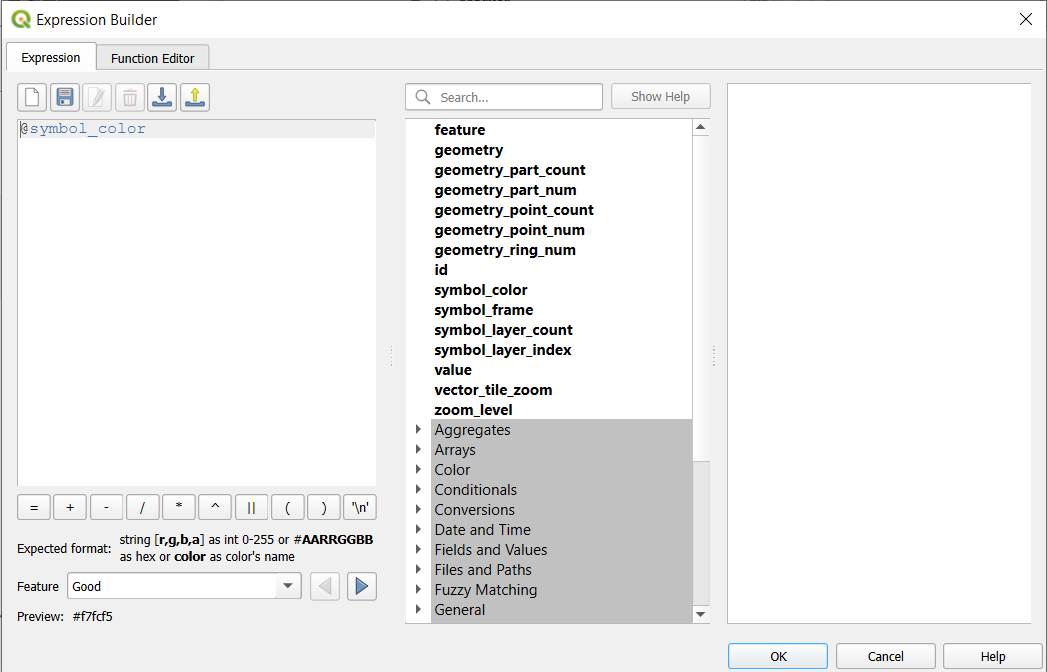
\includegraphics{./images/symbology_expressionbuilder.png}
\item
  click ``OK'' to apply and close the settings until you are back to the
  styles and then the map canvas, and you will see that what was a black
  ring around the points is now a ring the same color as the points
  themselves. 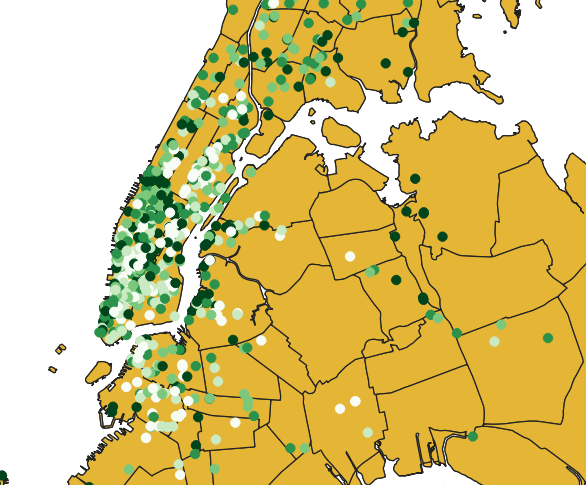
\includegraphics{./images/points_same_outline_as_fill.png}
\end{itemize}

While the above examples are for styling points, similar approaches can
be applied to lines and polygons as well.

*** Tips:

\begin{itemize}
\tightlist
\item
  Need to apply the same style to multiple similar layers with the same
  field name and similar value ranges? You can right click on a layer,
  navigate to \texttt{Styles} -\textgreater{} \texttt{Copy\ Style}
  -\textgreater{} \texttt{All\ Style\ Categories} and then right click
  on another layer, navigate to \texttt{Styles} -\textgreater{}
  \texttt{Paste\ Style} -\textgreater{} \texttt{All\ Style\ Categories}
  to save some work.
\end{itemize}

\begin{center}\rule{0.5\linewidth}{0.5pt}\end{center}

\hypertarget{raster-styling}{%
\subsection{Raster Styling}\label{raster-styling}}

Due to the nature of raster data compared to vector data, adjusting the
symbology is a bit different. In general, raster layers will default to
having a grayscale symbology applied, with darker shades for the lower
values and lighter for higher values, as you may have noticed for the
\textbf{Vegetation Density} dataset. In general, we may want to adjust
adjust the styling in various ways - the main thing to adjust is the
\textbf{Render Type} - you'll the following options:

\begin{itemize}
\tightlist
\item
  Multiband color - Generally for an image (a type of raster dataset),
  where, for example, there are different layers that represent red,
  green, and blue parts of the visible spectrum, and these layers can be
  merged visually to be what people might generally see (e.g., from an
  aerial image or satellite image).
\item
  Paletted/Unique Values - Typically for a categorical dataset, such as
  land cover data, where each pixel value represents a different type.
\item
  Singleband gray - The default for most raster datasets loaded in,
  where there is a single layer with values that can be represented
  along a continuous gradient (these can be integer or decimal, spanning
  positive and negative numbers).
\item
  Singleband pseudocolor - An option to apply various color gradients
  (including user-defined ones) to a singleband dataset such as
  described in the previous option.
\item
  Hillshade - Generally used to style elevation data in an aesthetically
  pleasing way that helps visualize the topography of the landscape.
\item
  Contours - Can be used to draw ``contour lines'' as are often applied
  on topographic maps, to delineate specific breaks along the landscape.
  While this is often used with elevation data, it can be used with
  other continuous variables, such as on air quality, soil moisture,
  etc.
\end{itemize}

In this example with the Vegetation Density raster, we will chose the
\emph{Singleband pseudocolor} option. If you expand the ``Min / Max
Value Settings'' portion of the menu, you can see a number of options -
the defaults are generally okay, but you can try adjusting these as
desired. If working with a dataset that has a known range and the values
for the color ramp do not meet the whole range, you may want to either
set ``User defined'' values or change the ``Accuracy'' option from
``Estimate (faster)'' to ``Actual (slower).'' As with before, I'm
adjusting the color ramp to be Greens, and then hitting ``OK.''

\begin{figure}

{\centering 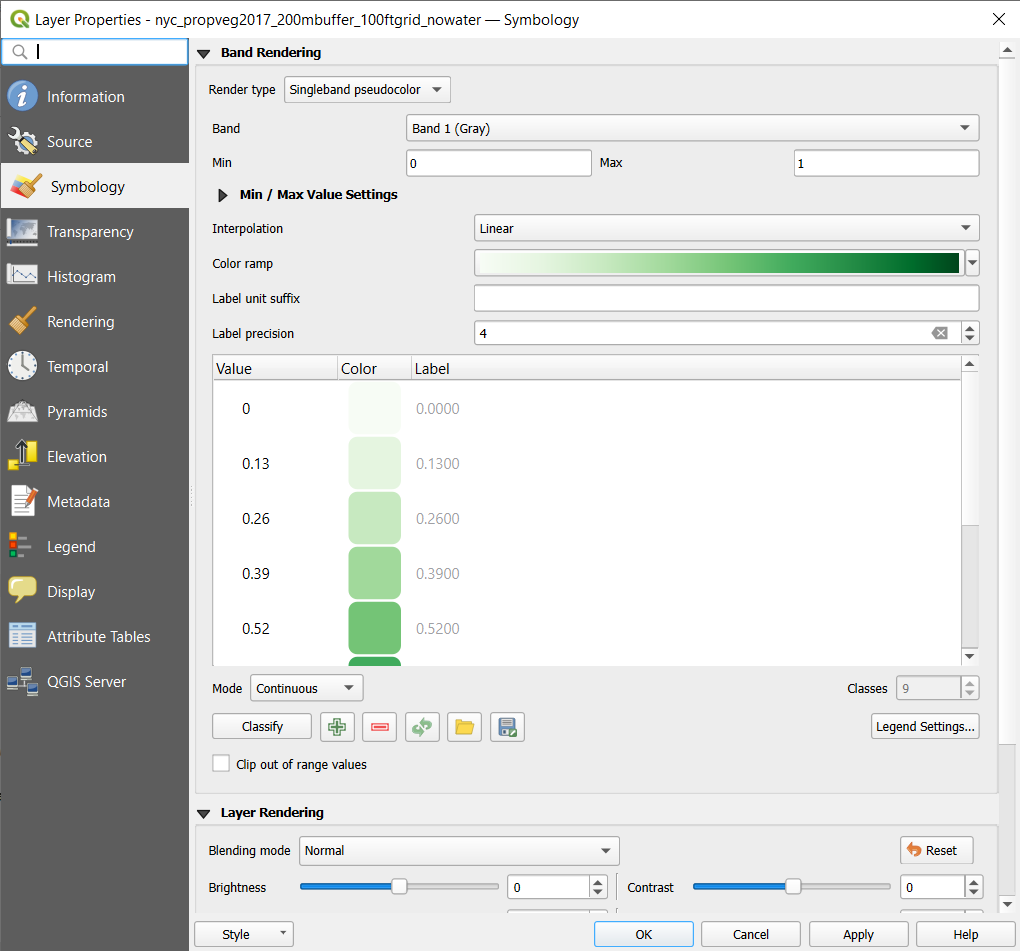
\includegraphics{./images/raster_style_greens.png}

}

\caption{Example of Layer Properties - Symbology menu for the Vegetation
Density raster dataset}

\end{figure}

The result should look along the lines of the following:

\begin{figure}

{\centering 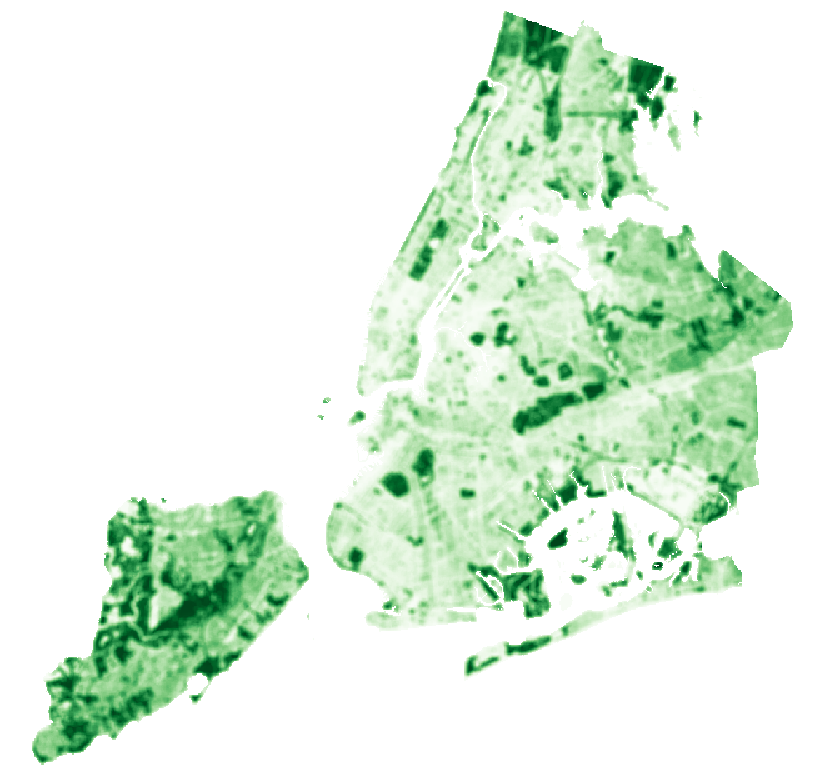
\includegraphics{./images/vegetation_density_greens.png}

}

\caption{Vegetation Density dataset with a green color gradient applied}

\end{figure}

Users can save and load style for layers, both for vector and raster
datasets. Included in the folder with the Vegetation Density data is a
\texttt{.qml} file that contains styling information used for the main
map in the
\href{https://medium.com/gage-nyc/looking-at-cooling-benefits-of-plants-through-nyc-vegetation-data-ccdeb33cbe17}{blog
post about that dataset} from the NYC Environmental Justice Alliance and
the The Nature Conservancy's NY Cities Program as part of the Just
Nature NYC partnership. From the Layer Properties - Symbology menu,
users can go to the ``Style'' button near the bottom, select ``Load
Style'' and set the File to use as
\texttt{vegmapping\_style\_qgis\_tutorial.qml} and click ``Load Style.''

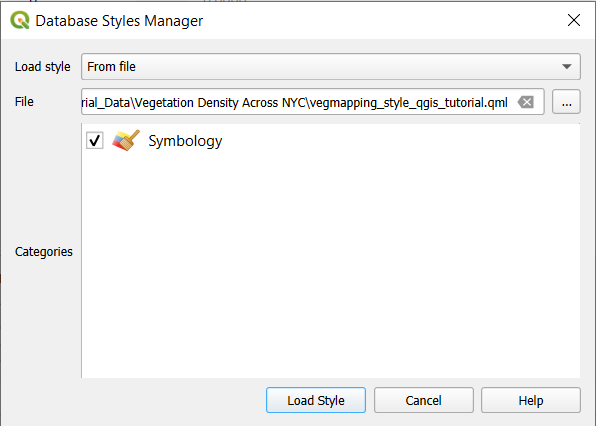
\includegraphics{./images/style_manager.png}

From there, simply clicking ``Apply'' or ``OK'' should yield a map that
looks like the below, where the transition from yellow to green happens
at the 0.32 mark, which is the proportion of land area within a 200
meter radius area that needs to be covered by vegetation to start
reducing air temperatures, based on research led by the NYC Department
of Health and Mental Hygiene.

\begin{figure}

{\centering 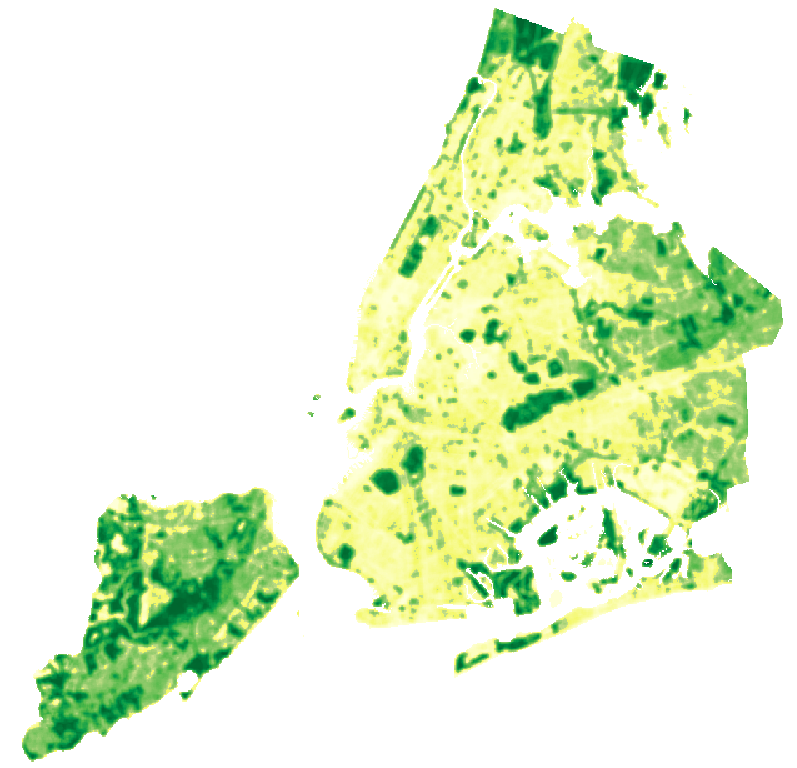
\includegraphics{./images/vegetation_density_custom.png}

}

\caption{Vegetation Density dataset with a yellow-greens gradient
applied based on a custom style loaded form a .qml file}

\end{figure}

\hypertarget{basemaps}{%
\subsection{Basemaps}\label{basemaps}}

In QGIS there are a few different ways to bring in basemaps. Users
familiar with different web services (e.g., WMS/WMTS, ArcGIS REST
services, etc.) can specify those through the Data Source Manager or the
Browser panel, but more simply, for many use cases, users can use the
\textbf{QuickMapServices plugin}. If it is not already up, you can click
the \includesvg{index_files/mediabag/mActionSearch.svg} on the toolbar.
From there, in the SearchQMS panel, users can search for various
basemaps, such as from Google. Note, these are not necessarily licensed
openly for broad reuse, but for visualizing datasets together, this can
still be useful! Additionally, if you search for ``nyc.gov'' you can
find basemaps, labels, and imagery specific to NYC from the City of New
York, and acceptable for use in various ways under a Creative Commons
license - see the \href{https://maps.nyc.gov/tiles/}{associated
website}. To load a given basemap into QGIS, users can double-click an
entry, or click the ``Add'' button; the layers get added to the bottom
of the list of layers in the Layers panel.

\begin{figure}

{\centering 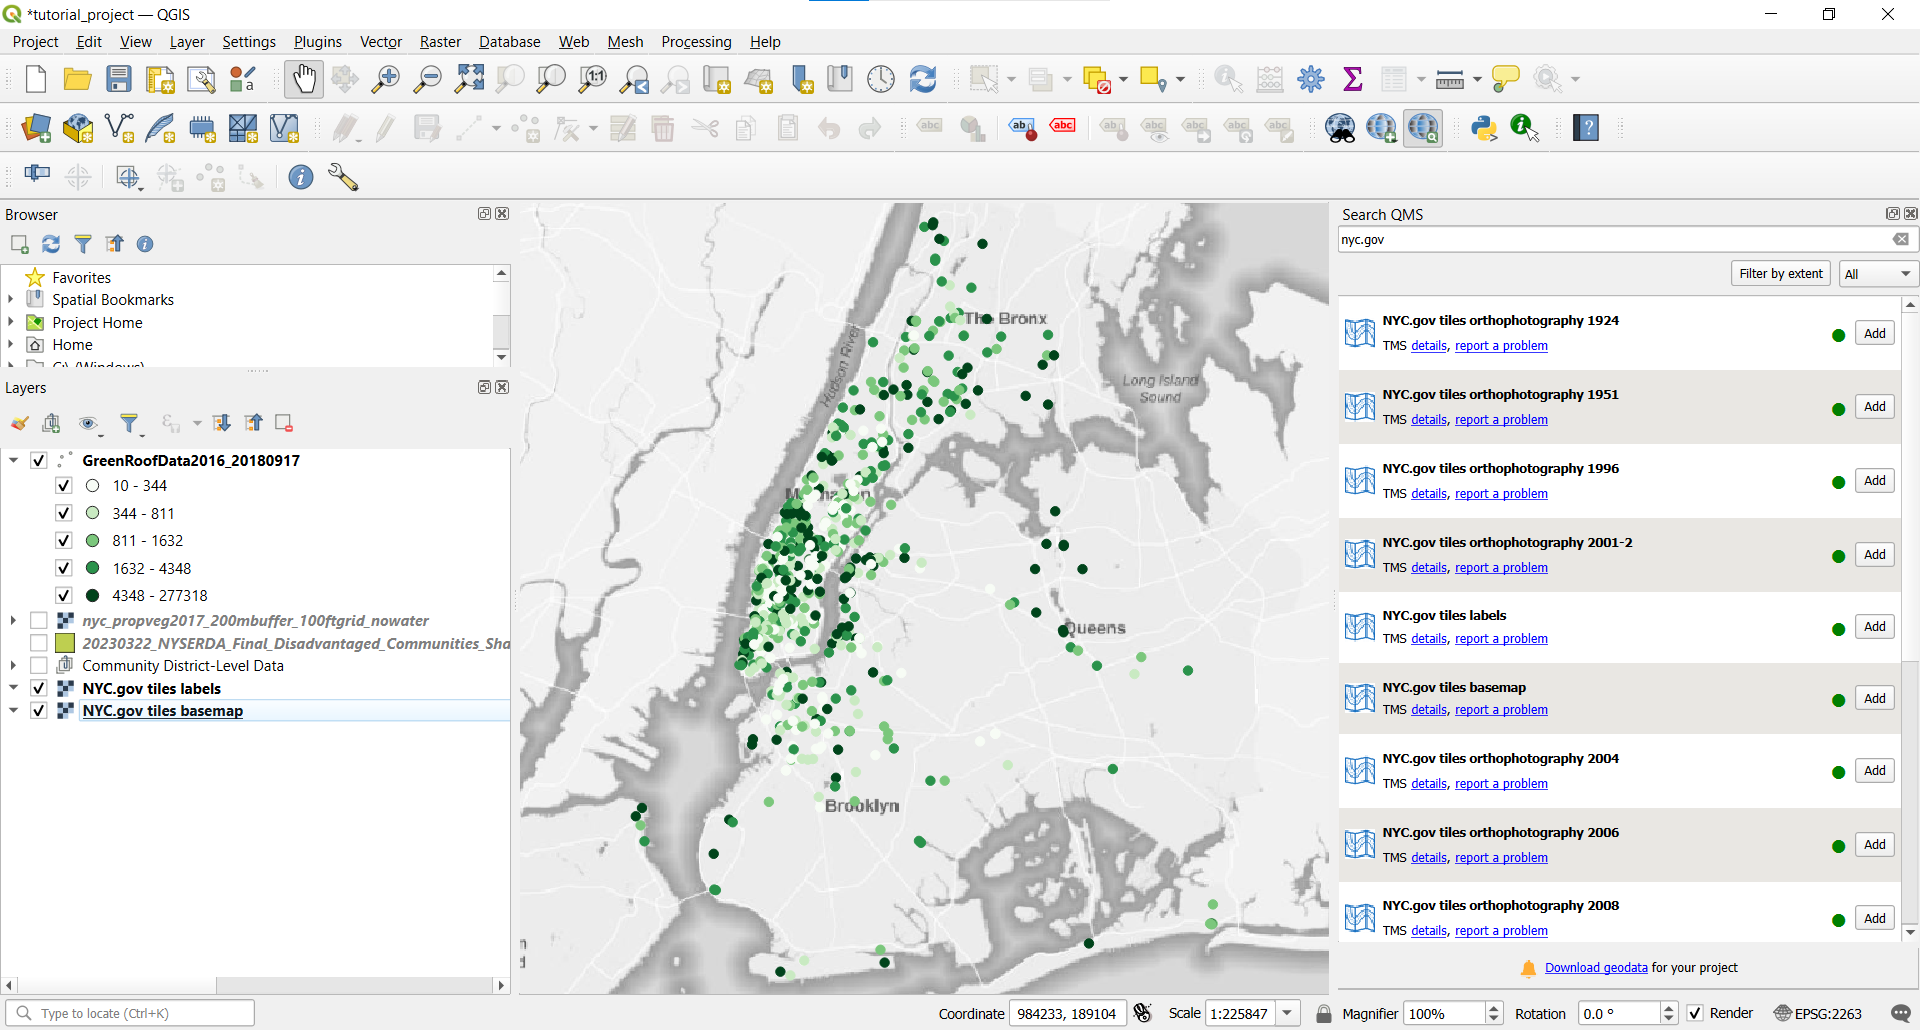
\includegraphics{./images/qms_nyc_basemap.png}

}

\caption{Example of the Green Roof Centroid data mapped over a basemap}

\end{figure}

\bookmarksetup{startatroot}

\hypertarget{projections}{%
\chapter{Coordinate Reference Systems}\label{projections}}

Geographic datums, projections, and coordinate systems, jointly making
up Coordinate Reference Systems (CRSs) are each big topics. This chapter
is not even intended to be a primer about the topics themselves, but
rather to help new QGIS users, or new GIS users more generally, get
started in GIS operationally.

\textbf{\emph{Note: In general, to do spatial data processing with two
or more layers, the data layers need to be in the same CRS. If the data
were not already available in the same CRS, they can be transformed to
be in a common CRS as described in this section.}}

\hypertarget{checking-and-setting-project-and-layer-crs}{%
\section{Checking and Setting Project and Layer
CRS}\label{checking-and-setting-project-and-layer-crs}}

QGIS automatically reads Coordinate Reference System information, if
available, from data layers. For shapefiles, it generally relies on the
\texttt{.prj} sidecar file; for most other vector formats and raster
data, it is generally embedded in the file. If you load data without
built-in projection information (e.g., a Delimited Text File), it
generally assumes a geographic coordinate system - either
Latitude/Longitude in the WGS 84 datum (\href{https://epsg.io/4326}{EPSG
4326}) or the Project CRS, generally defined based on the first dataset
loaded for a project unless otherwise specified by the user.

To see what the Project CRS is, you can check the bottom-right corner of
the main QGIS window and it will indicate next the
\includesvg{index_files/mediabag/mIconProjectionEnabl.svg} - you can
click . Alternatively, go to the \texttt{Project} menu at the top of the
QGIS window, select \texttt{Project\ Properties} and then select the CRS
tab on the side. In the tutorial project I set up for myself in working
through this tutorial, the Project CRS is NAD83 / New York Long Island
(ftUS), with a shorthand code, the EPSG code, being 2263
(\href{https://epsg.io/2263}{EPSG 2263}). For the data in this tutorial,
this is a good, locally-appropriate CRS.

\begin{figure}

{\centering 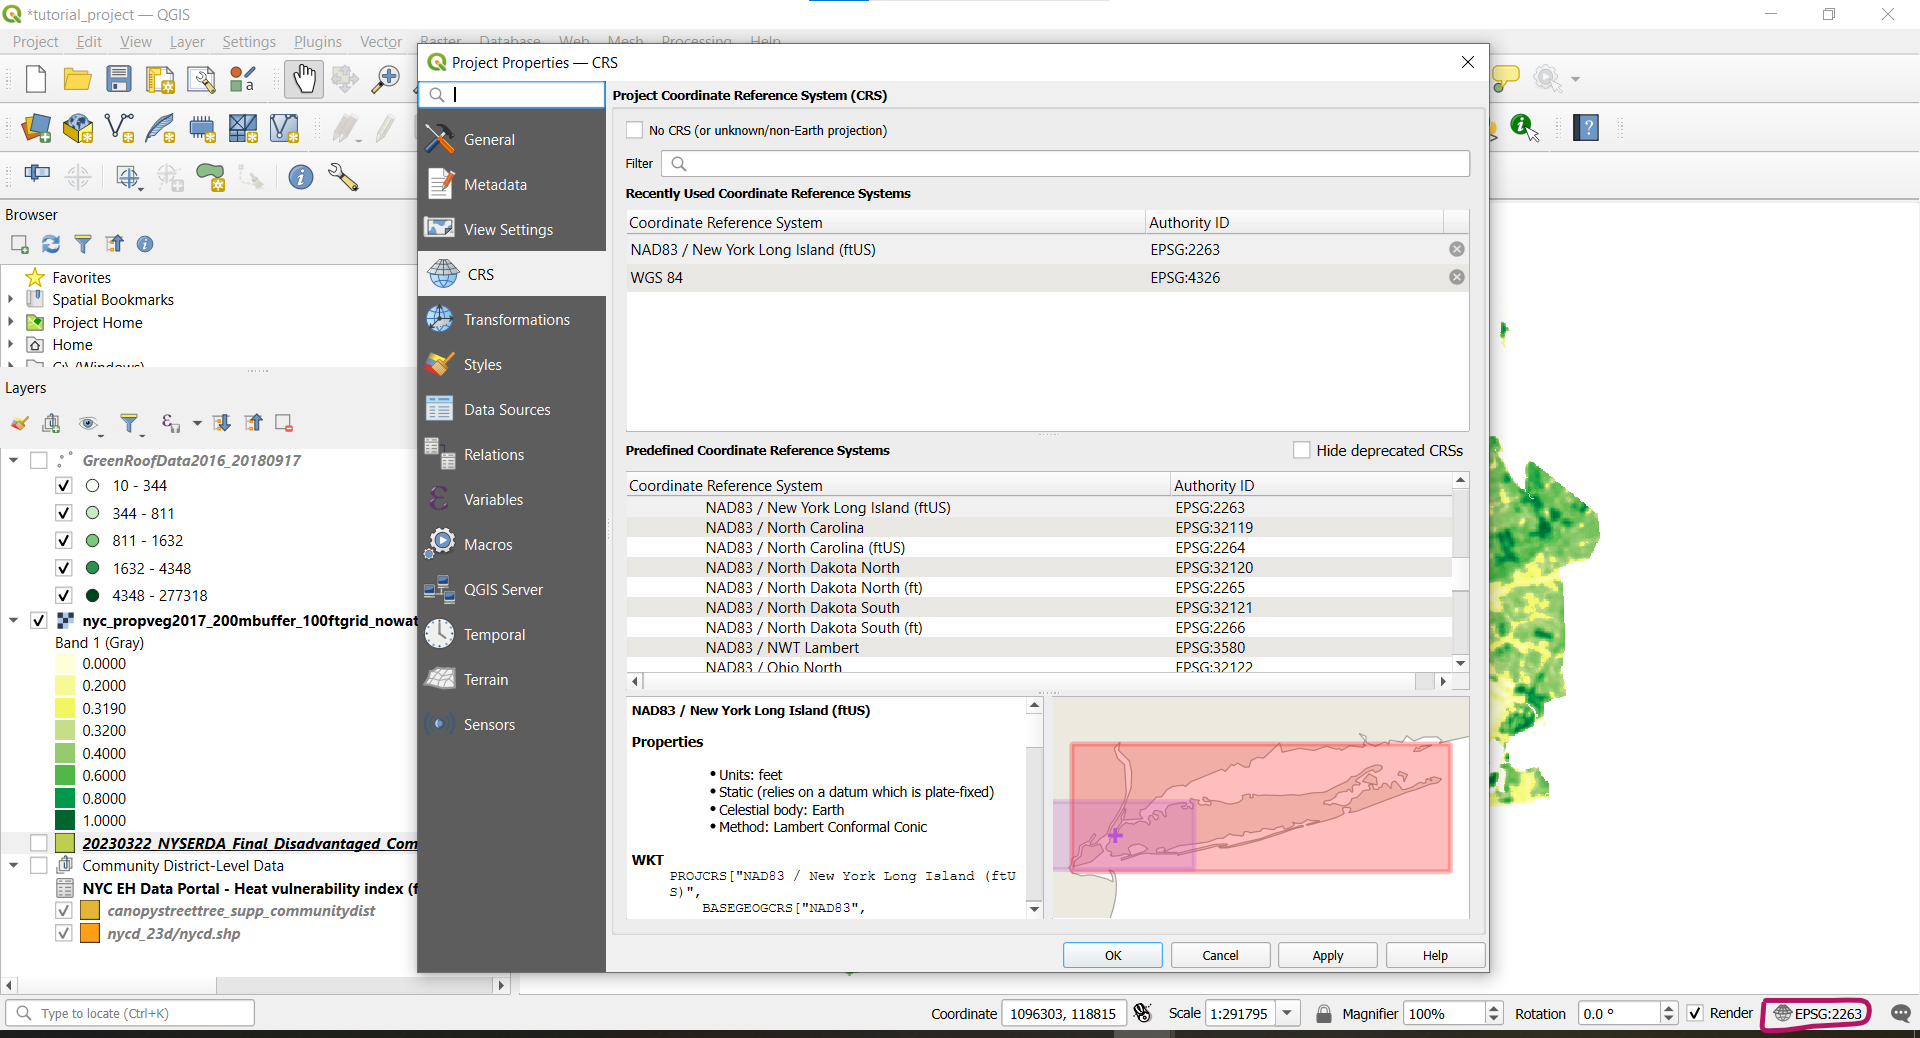
\includegraphics{./images/project_crs.png}

}

\caption{Example of looking at the Coordinate Reference System for a
project, showing in this case, the Project CRS is NAD83 / New York Long
Island (ftUS), EPSG 2263. Clicking on the area circled in Purple in the
main QGIS window is a shortcut to get to the Project Properties - CRS
window, shown here in the foreground.}

\end{figure}

To check what CRS QGIS is using for a layer, the quickest way is to
right-click on a layer, and hover over ``Layer CRS'' - the top item in
what appears is the CRS that QGIS is using. From here, users can change
the Project CRS to that of the layer, or change it. Note, ``setting''
the layer CRS is simply telling QGIS how to interpret the coordinates
associated with the spatial data. If the data are not actually in the
CRS being assigned, things will not appear to be in the right places.

\begin{figure}

{\centering 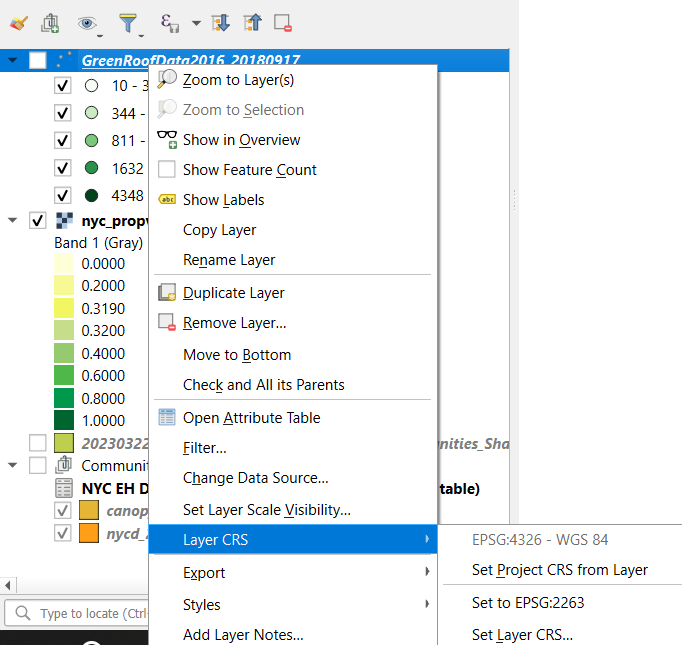
\includegraphics{./images/CheckLayerCRS.png}

}

\caption{Checking the layer CRS for the Green Roof Centroid data}

\end{figure}

\hypertarget{on-the-fly-projection}{%
\subsection{On the Fly Projection}\label{on-the-fly-projection}}

QGIS and most other GIS software has what is called \emph{On the Fly
Projection} meaning that data do not need to be in the same CRS to be
\emph{viewed} together in the correct place. Basically, the necessary
mathematical transformations are conducted by the software as needed to
support visualizing all of the data together. To see what things might
look like if this was not the case, you can go to the Project CRS
information as shown above, and check the box at the top for ``No CRS
(or unknown/non-earth projection)'' and then use the
\includesvg{index_files/mediabag/mActionZoomFullExten.svg} in the
toolbar to zoom to the full extent all of the layers at once. What you
see will likely look \emph{very} zoomed out, and you will see some data,
quite small, and far apart from one-another, and maybe not see others
because they are so small when plotted on common units, rather than
re-projected on the fly so everything lines up.

To get back to how things were, go back to the Project CRS, uncheck the
box you just checked, select the appropriate CRS (EPSG 2263 in this
case), and click ``OK.''

\hypertarget{transforming-to-a-different-crs---vector-data}{%
\section{Transforming to a Different CRS - Vector
Data}\label{transforming-to-a-different-crs---vector-data}}

Per the note at the beginning of this section, data layers should
generally be in the same CRS for spatial processing operations (any way
in which you are using the data together, spatially, beyond
visualization). While EPSG 2263 is a generally suitable CRS for work in
NYC, not all of the layers shared with this tutorial are in this CRS; in
particular, the following are in different CRSs - Green Roof Centroids
data (in Latitude/Longitude coordinates according to the WGS84 datum)
and the Disadvantaged Communities Data (in UTM zone), thus they should
be transformed to align with the CRS of the other layers.

In QGIS transform vector to a different CRS, or ``reprojecting'' the
data is generally done through an export operation, where the spatial
data are transformed to in the process of the export. To start,
right-click on a layer, navigate to ``Export'' and select ``Save
Features As.''

\begin{figure}

{\centering 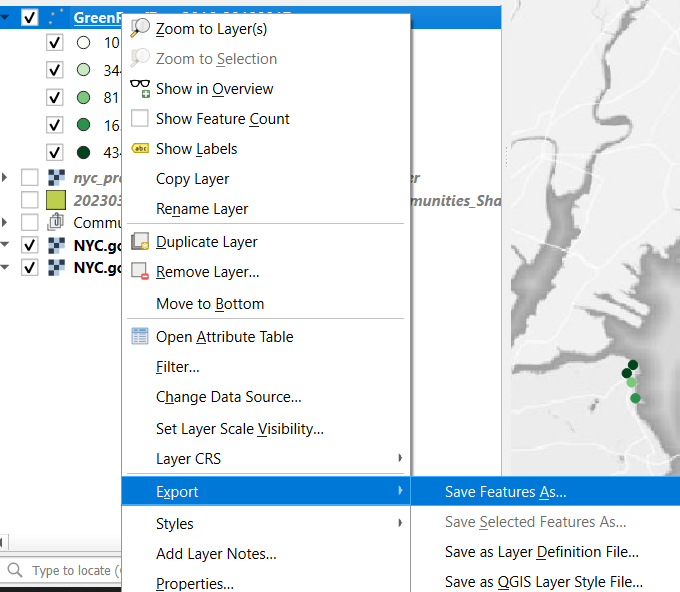
\includegraphics{./images/export_vector_1.png}

}

\caption{Navigating to vector layer export menu}

\end{figure}

In the menu that pops up, you can chose from different formats; in this
case I will select GeoPackage (\texttt{.gpkg} extension), an open
standard format that can have multiple layers within a single file. For
my tutorial project, I'll create a single where I will save my outputs.
You can set the destination file location and name for the GeoPackage
file, and specify the layer name, which will default to the same name as
the original. For work like this, I tend to adjust the layer name to
reflect the important change, and I add ``\_epsg2263'' to the end of the
default. Then, most importantly, for CRS, you should be able to select
\emph{EPSG:2263} from the dropdown menu for CRS, but if you don't, you
can search for it and select it via the
\includesvg{index_files/mediabag/mActionSetProjection1.svg} icon to the
right of that. From there, generally the defaults for the export can be
left as-is, leave the box checked at the bottom to ``Add saved file to
map'' and click ``OK.''

\begin{figure}

{\centering 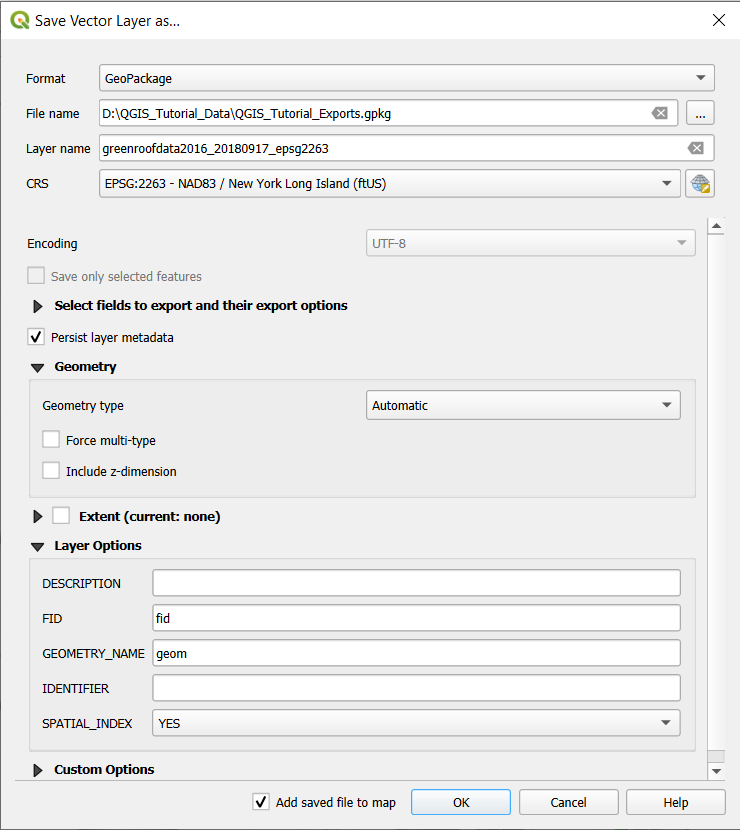
\includegraphics{./images/export_vector_2.png}

}

\caption{Sample dialogue box for exporting the Green Roof Centroid data
while transforming the data to the desired CRS}

\end{figure}

\textbf{\emph{Before proceeding in this tutorial, please reproject the
Disadvantaged Communities dataset}}

Some notes for after export:

\begin{itemize}
\tightlist
\item
  When the layer is loaded upon export, the default name for GeoPackage
  layers can be rather long, thus you may wish to rename to a shorter
  but intuitive name;
\item
  As data are exported and re-imported, the layer styling is lost. Thus,
  you may wish to right click on the original layer, navigate to copy
  the layer styles, and then paste them to the new, reprojected version;
\item
  With the new version of the layer loaded, you may want to remove the
  old version - you can do this by clicking on it and then using the
  \includesvg{index_files/mediabag/mActionRemoveLayer.svg} icon at the
  top of the Layers panel, or by right-clicking on the layer and
  selecting ``Remove Layer.''
\end{itemize}

\hypertarget{transforming-to-a-different-crs---raster-data-coming-soon}{%
\section{Transforming to a Different CRS - Raster Data (Coming
Soon!)}\label{transforming-to-a-different-crs---raster-data-coming-soon}}

For the raster data in this tutorial, with the analyses described,
reprojection of the raster is not necessary. However, for completeness,
a walk-through of accomplishing this is pending.

\bookmarksetup{startatroot}

\hypertarget{working-with-multiple-datasets-together}{%
\chapter{Working with Multiple Datasets
Together}\label{working-with-multiple-datasets-together}}

The world of spatial data operations is vast! Some examples of working
with multiple data layers or tables are included here as examples. In
some cases, adjustments could be made in the workflows shown based on
different needs or preferences. And there are countless other operations
that could be done with the tutorial datasets alone.

As you work through the below processes, take some time to re-style
applicable datasets to see what the results look like, and think about
potential implications in terms of the distribution of things like green
roofs, and vegetation more broadly, in New York City.

\hypertarget{tabular-joins}{%
\section{Tabular Joins}\label{tabular-joins}}

In many cases data are made available for common administrative or
political geographic units. For example, in the United States, data are
often made available by units such as, from larger units to (generally)
smaller, State, County, City, Census Tracts. In New York City, a number
of datasets are released at the scale of
\href{https://www.nyc.gov/site/planning/community/community-portal.page}{Community
Districts}; each Community District has a Board that weights in on a
variety of types of issues, and serves as a space for broader public
engagement from the associated geographic area.

Community District boundaries for New York City, made available by the
Department of City Planning, are one of the datasets shared with this
tutorial. Both the Heat Vulnerability Index data, which is a non-spatial
data table, and the Tree Canopy and Street Tree Summary data with the
tutorial data are available for Community Districts. Thus, we should be
able to associate data from these different datasets together, or
``join'' them based on the unique identifier for each Community
District. In this case, because the Community District Boundaries as
made available from the NYC Department of City Planning are the
simplest, in that they primarily have the spatial polygon data and the
Community District identifiers, we will join these other datasets to it.
In the working project for this demo, the layer name for the Community
District Boundaries is ``nycd\_23d/nycd.shp'' (the default name from
dragging and dropping the \texttt{.zip} folder with the data into QGIS).
Before going through the below steps, I have looked at the attribute
tables to find that:

\begin{itemize}
\tightlist
\item
  In the Heat Vulnerability Index data table, the Community District
  identifier is coded in the column (field) \texttt{borocd}.
\item
  In the Tree Canopy and Street Tree Summary data for Community
  Districts, the Community District identifier is in the field
  \texttt{borocd}.
\item
  In the Community District Boundaries dataset, the Community District
  identifier is in the field \texttt{BoroCD}.
\end{itemize}

To create the tabular join to associate the Heat Vulnerability Index
with the Community District boundaries:

\begin{itemize}
\tightlist
\item
  Go to the Layer Properties window for the Community District
  Boundaries.
\item
  Click on the ``Joins'' tab on the left side of the window.
\item
  Click the \includesvg{index_files/mediabag/mActionAdd1.svg} at the
  bottom.
\item
  As the ``Join layer'' specify the Heat Vulnerability Index dataset.
\item
  For the ``Join field,'' or column of data from the dataset being
  joined to the Community District Boundaries, specify the field that
  has the Community District identifiers (\texttt{borocd})
\item
  Specify the ``Target field,'' or the field that the Heat Vulnerability
  Index dataset is being joined to, as \texttt{BoroCD}
\item
  In this case, we may do not really need any fields other than the
  index itself, or the ``Score'' so we can check the box next to
  ``Joined fields'' and then check the box next to the desired field.
\item
  Click ``OK'' in the Joins window and then in the Layer Properties to
  get back to the main QGIS window.
\item
  Open the attribute table for the Community District Boundaries and see
  if it worked!
\end{itemize}

\begin{figure}

{\centering 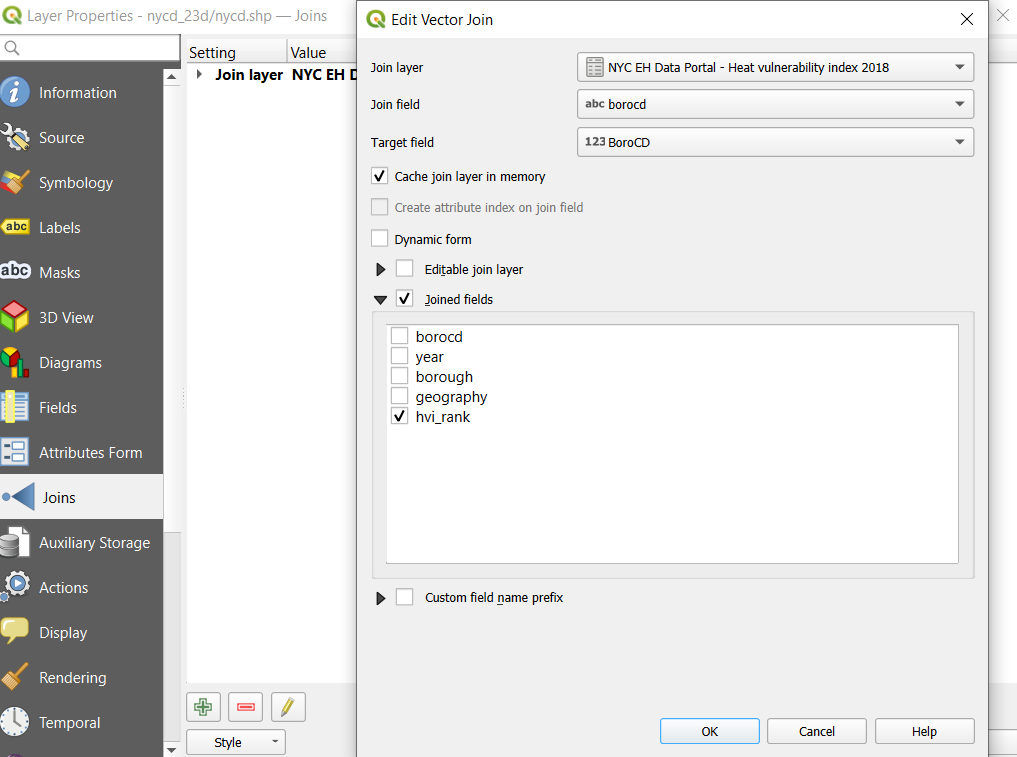
\includegraphics{./images/TabularJoin.png}

}

\caption{Setting up the join between the Heat Vulnerability Index data
and the Community District Boundaries}

\end{figure}

And when we look at the attribute table for the Community District
Boundaries, we see a column with the Heat Vulnerability Index rank.
(Some rows have no entry, which is expected as those rows are for
unpopulated areas, such as large parks and airports.)

\begin{figure}

{\centering 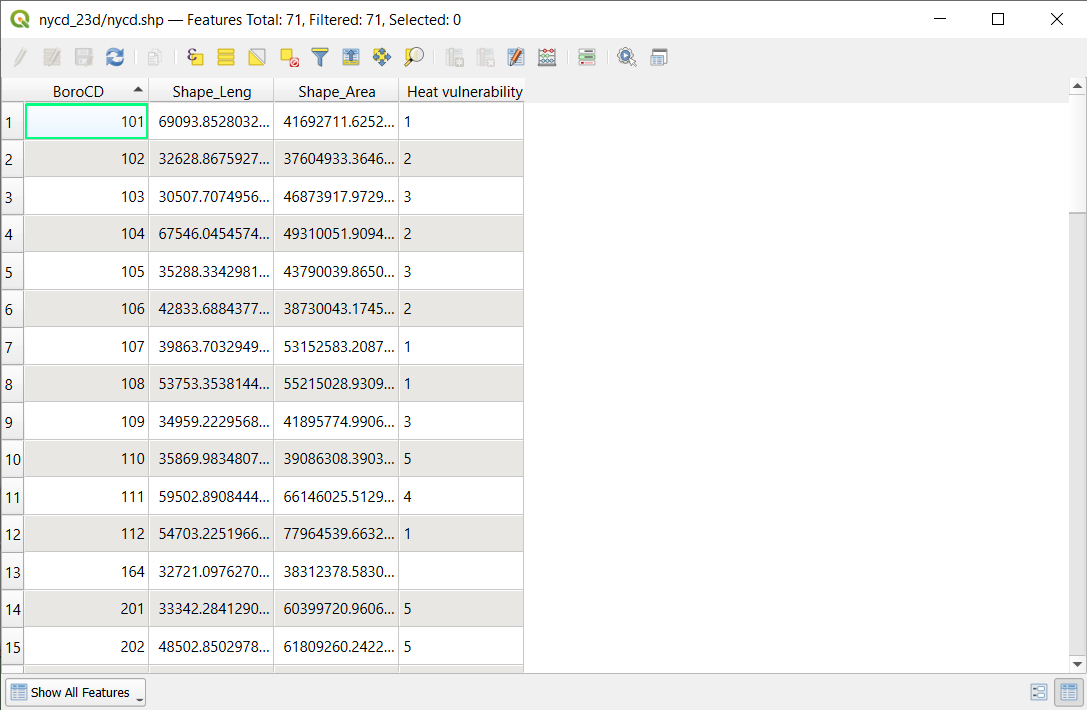
\includegraphics{./images/HVI_CD_Join_Result.png}

}

\caption{Attribute table of the Community District Boundaries layer
after joining the Heat Vulnerability Data based on the Community
District identifier}

\end{figure}

\hypertarget{saving-tabular-join-results}{%
\subsection{Saving Tabular Join
Results}\label{saving-tabular-join-results}}

Tabular joins accomplished through the above steps are only stored ``in
memory'' until exported While they will be maintained when the project
is saved, it is necessary to export the Community District Boundaries
dataset as a new dataset to have the joined data more permanently
available with that dataset.

There are multiple ways to do tabular joins in QGIS; there is another
workflow that can result in directly exporting the results to a new
layer. You can find that as the \textbf{Join Attributes by Field Value}
tool in the Processing Toolbox.

\hypertarget{try-it-yourself}{%
\subsection{Try it yourself!}\label{try-it-yourself}}

\textbf{\emph{As another tabular join, try to join the Tree Canopy and
Street Tree summaries by Community District to the Community District
Boundaries (with the Heat Vulnerability Index already joined). The
dataset is large - consider only keeping one or two fields of interest
from the Tree Canopy and Street Tree summary data.}}

\hypertarget{spatial-joins}{%
\section{Spatial Joins}\label{spatial-joins}}

One of the most valuable aspects of GIS software is the ability to
integrate different spatial datasets. In this case, for example, we can
associate something like the Community District identifier with each
green roof, or we can count the number of green roofs per Community
District. Lets do both!

\hypertarget{associating-broader-data-with-local-data}{%
\subsection{Associating Broader data with Local
Data}\label{associating-broader-data-with-local-data}}

With the data available with this tutorial, we can do a spatial join to
add information on Community District (e.g., which Community District)
to the individual green roof points. We will use the \textbf{Join
Attributes by Location} tool from the Processing Toolbox.

\begin{itemize}
\tightlist
\item
  Set the ``Join to features in'' to the green roof dataset
\item
  For the ``Features they (geometric predicate)'' - this is basically
  the place to specify what kind of relationship we are looking for
  between the green roof points and the Community District boundaries.
  In this case, we want information based on where the green roof points
  \emph{are within} the Community District boundaries.
\item
  The only field of interest in this case to add onto the Green Roof
  Data is the Community District identifier (\texttt{BoroCD}).
\item
  Set the ``Join Type'' to ``Create separate feature for each matching
  feature (one-to-many)''

  \begin{itemize}
  \tightlist
  \item
    Basically this is to specify that should there be instances where
    the boundary dataset had overlapping polygons, if multiple polygons
    overlapped with a green roof point, the output would have multiple
    entries for that green roof point, each with the respective
    Community District (in this case) identifier. This is not an issue
    in this case, but could be with different datasets.
  \end{itemize}
\item
  In the screenshot below I have left it so the result is only written
  out as a ``Temporary layer'' but you could opt to use the icon to the
  left of that box to specify a destination file.
\item
  Click ``Run''!
\end{itemize}

\begin{figure}

{\centering 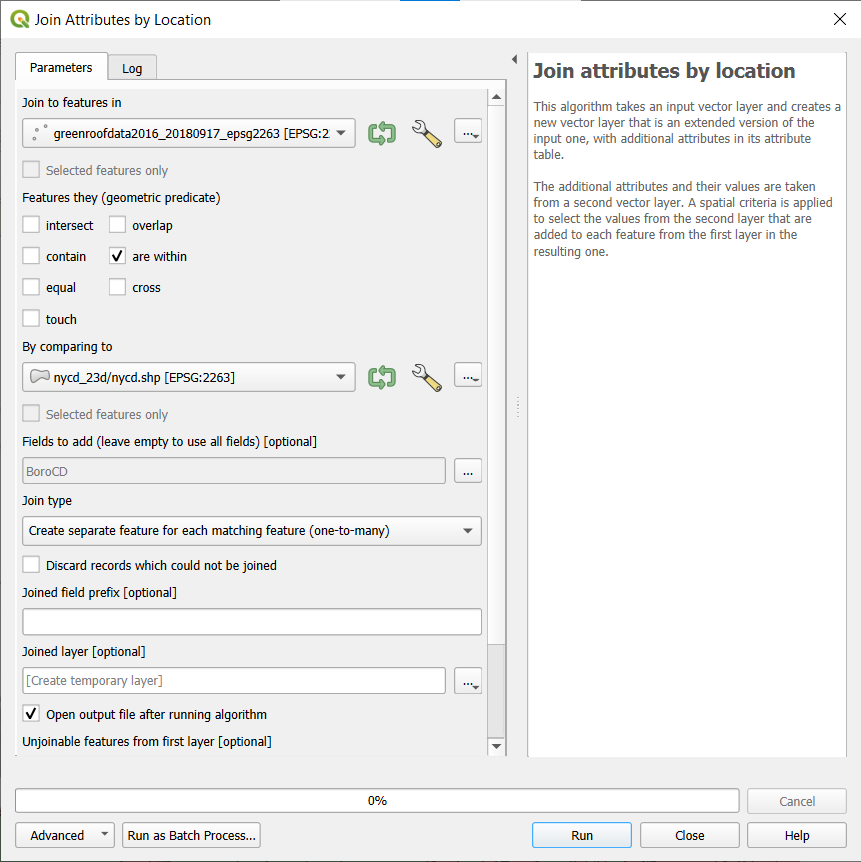
\includegraphics{./images/CommDist_to_GreenRoofs_Setup.png}

}

\caption{Setting up a spatial join to get information about Community
Districts associated with the Green Roof Centroids}

\end{figure}

After this runs, you will see a new result in the Layers panel, ``Joined
layer,'' with an associated dataset shown on the map canvas. The
attribute table should include both the fields from the original Green
Roof Centroid data, as well as the Community District identifier.

\hypertarget{summarizing-local-data-to-larger-areas}{%
\subsection{Summarizing Local data to Larger
Areas}\label{summarizing-local-data-to-larger-areas}}

In many cases we may want to count the number of something within
geographic units. In this case, we can count how many green roofs are in
each Community DIstrict. To do this, we use the \textbf{Join Attribute
by Location (Summary)} tool from the Processing Toolbox.

\begin{itemize}
\tightlist
\item
  Specify the ``Join to features in'' dataset as the Community District
  boundaries.
\item
  Check the box for ``contain'' for ``Where the features.''
\item
  Set the ``By comparing to'' dataset as the Green Roof Centroid data
  (make sure to use the version reprojected to EPSG 2263).
\item
  For ``Fields to summarise'' if you leave this out, you will end up
  with the desired summary statistics for all of these fields. Thus, I
  have selected only the unique identifier field, \texttt{fid}.
\item
  For ``Summaries to calculate'' - if you leave blank, it will calculate
  all possible summaries. I selected ``Count'' as the metric of
  interest.
\item
  Again, you can opt to write the output to a permanent file, or leave
  the default to create a temporary layer.
\end{itemize}

\begin{figure}

{\centering 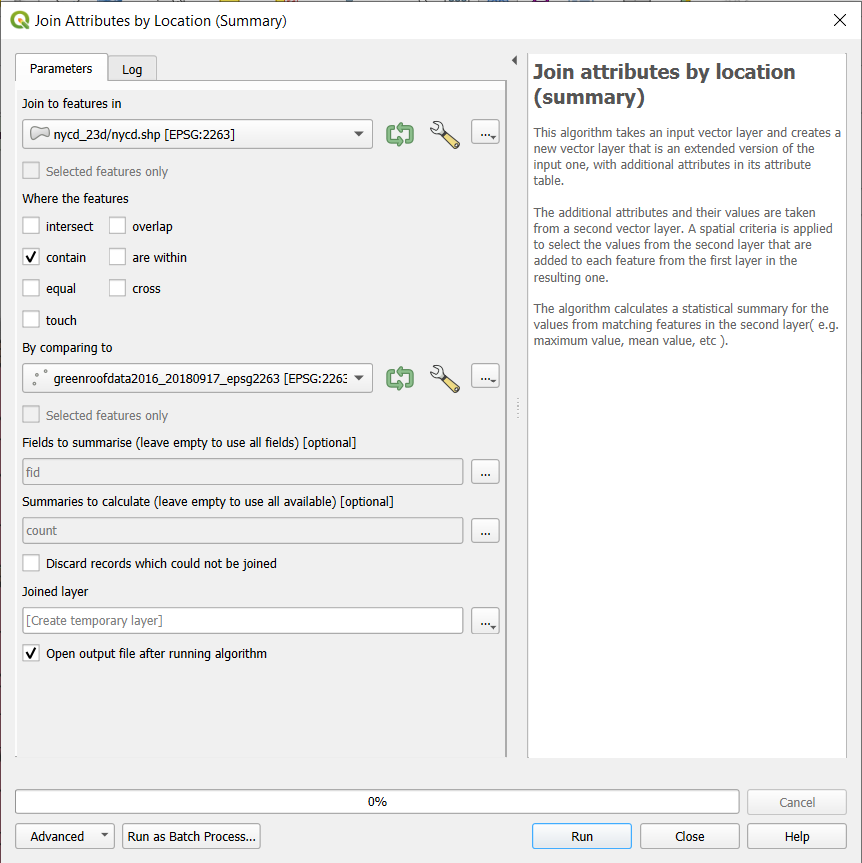
\includegraphics{./images/count_points_setup.png}

}

\caption{Setting up spatial join to count the number of Green Roofs,
based on their centroids, within each Community District}

\end{figure}

As with the previous operation, you should see a result of a ``Joined
layer'' and see a new field reflecting the count of green roofs, as well
as the fields originally in the Community District Boundaries dataset.

\hypertarget{raster-polygon-overlays}{%
\section{Raster-Polygon Overlays}\label{raster-polygon-overlays}}

In many cases it may be of interest to aggregate information from a
raster data layer to a broader set of spatial boundaries. With the
tutorial data, we calculate metrics from the Vegetation Density data by
Community District - for example, to understand how the different
Community Districts may have higher average values for vegetation
density than others. To do this, we'll use the \textbf{Zonal Statistics}
tool from the Processing Toolbox, which calculates statistics of a
raster layer for each feature of an overlapping polygon layer.

\begin{itemize}
\tightlist
\item
  Specify the Input layer as the COmmunity District Boundaries.
\item
  Specify the Raster Layer as the Vegetation Density raster.
\item
  We can specify a prefix for the new columns that will be created to
  help ease remembering what the new columns will have been created from
  (e.g., ``PropVeg\_'').
\item
  We can specify a variety of statistics to calculate; in this case,
  I've specified that the the Mean and Median vegetation density values
  should be calculated for each Community District.
\item
  Click ``Run''!
\end{itemize}

\begin{figure}

{\centering 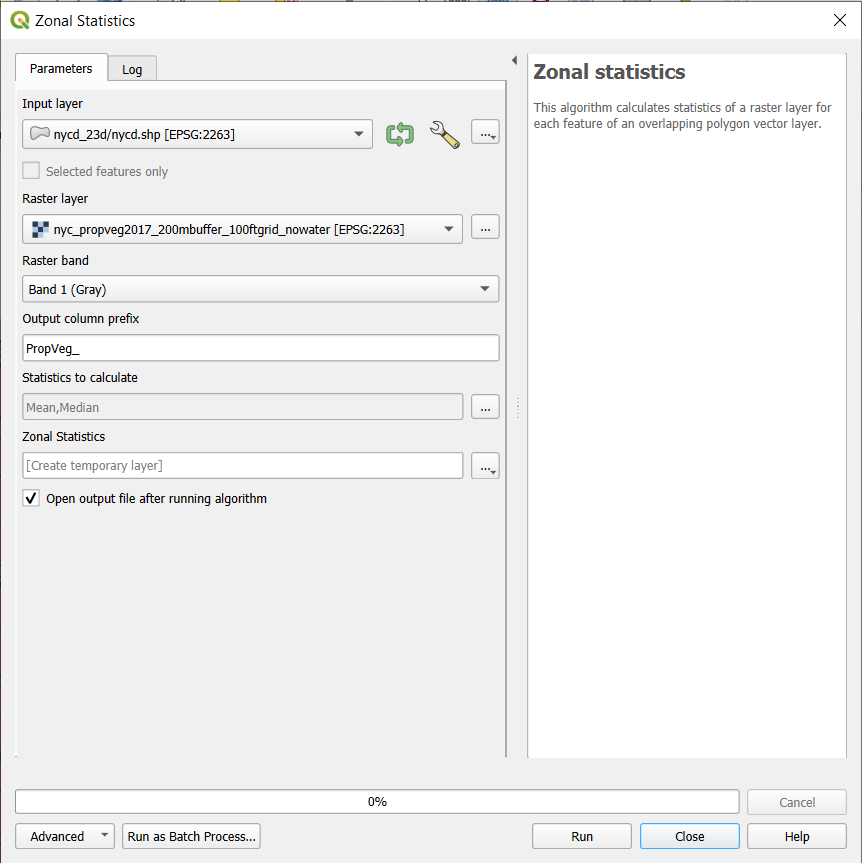
\includegraphics{./images/ZonalStatsSetup.png}

}

\caption{Setting up a Zonal Statistics operation to calculate summary
statistics from the Vegetation Density data layer for each Community
Districts}

\end{figure}

You should see a new layer titled ``Zonal Statistics'' with fields
reflecting the Mean and Median values for the Vegetation Density layer.

\hypertarget{clipping}{%
\section{Clipping}\label{clipping}}

In many cases, we have access to datasets that are much broader than our
area of interest. For example, the Disadvantaged Communities Dataset is
for the entirety of New York State, and the Census Tracts in it for NYC
include the water areas of New York Harbor. Thus, this is a great
example of a dataset that could be clipped to New York City.

First - as a look of what the dataset should look like (this version has
been reprojected to EPSG 2263).

\begin{figure}

{\centering 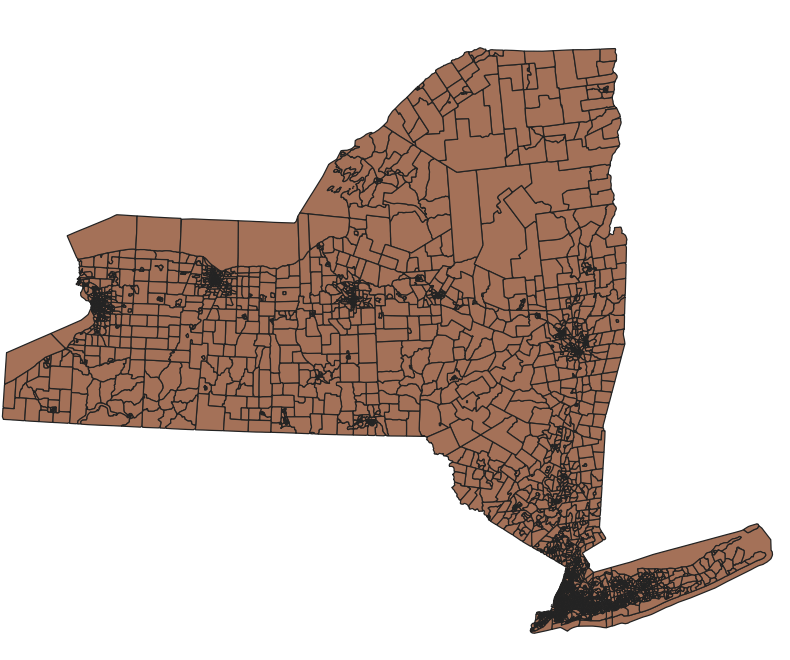
\includegraphics{./images/DisadvantagedCommunities_StateWide.png}

}

\caption{The full Disadvantaged Communities Dataset for New York State}

\end{figure}

We can clip the dataset to the Community District Boundaries data layer
using the ``Clip'' tool under the ``Vector Overlay'' heading in the
Processing toolbox.

The dialogue box for the Clip tool is fairly simple, only asking for the
Input layer (data that we want to clip) and the Overlay layer, or the
dataset that we want to clip to. After clicking ``Run'' you should end
up with a new result layer, ``Clipped'' that looks like this:

\begin{figure}

{\centering 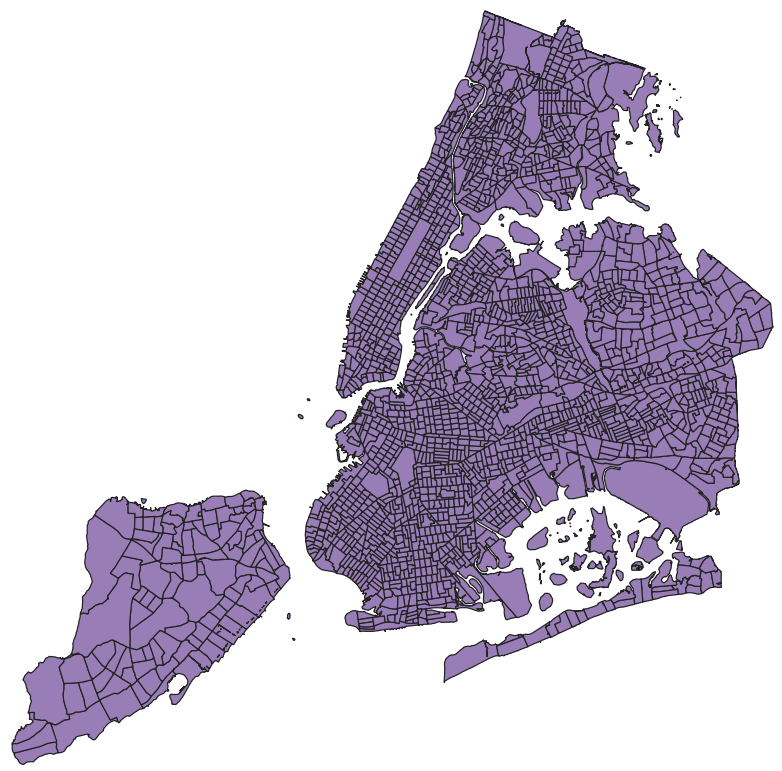
\includegraphics{./images/DisadvantagedCommunities_Clipped.png}

}

\caption{The result of clipping the Disadvantaged Communities Dataset to
the NYC Community District Boundaries}

\end{figure}

\bookmarksetup{startatroot}

\hypertarget{making-maps}{%
\chapter{Making Maps}\label{making-maps}}

Of course GIS is not just about looking at data on your computer\ldots{}
its about sharing it with the world through maps! There's a lot that one
can do in terms of cartography in QGIS, and though not covered in this
tutorial, you can even make interactive, web-based maps using the
\textbf{QGIS2Web}, to post on a website, or even just share the files
with others to explore the data themselves.

\hypertarget{qgis-layouts}{%
\section{QGIS Layouts}\label{qgis-layouts}}

Cartography in QGIS is mainly done through the \textbf{Layouts} window
and respective set of tools. You can start creating a new print layout
by clicking \includesvg{index_files/mediabag/mActionNewLayout.svg}
towards the upper-left of toolbar in QGIS - if you do so, you will be
prompted to name the layout. You can also click the Layout Manager icon
\includesvg{index_files/mediabag/mActionLayoutManager.svg}, which will
let you see what other layouts, if any, you've already created and
create new ones, among other things.

After clicking \includesvg{index_files/mediabag/mActionNewLayout.svg}
and entering a name for a new layout, a new window will open - you may
need to maximize it depending on your own computer. Once there, you can
right-click on the blank white area, and select ``Page Properties'' to
adjust things like the background color to be working with, and the
paper size.

\begin{figure}

{\centering 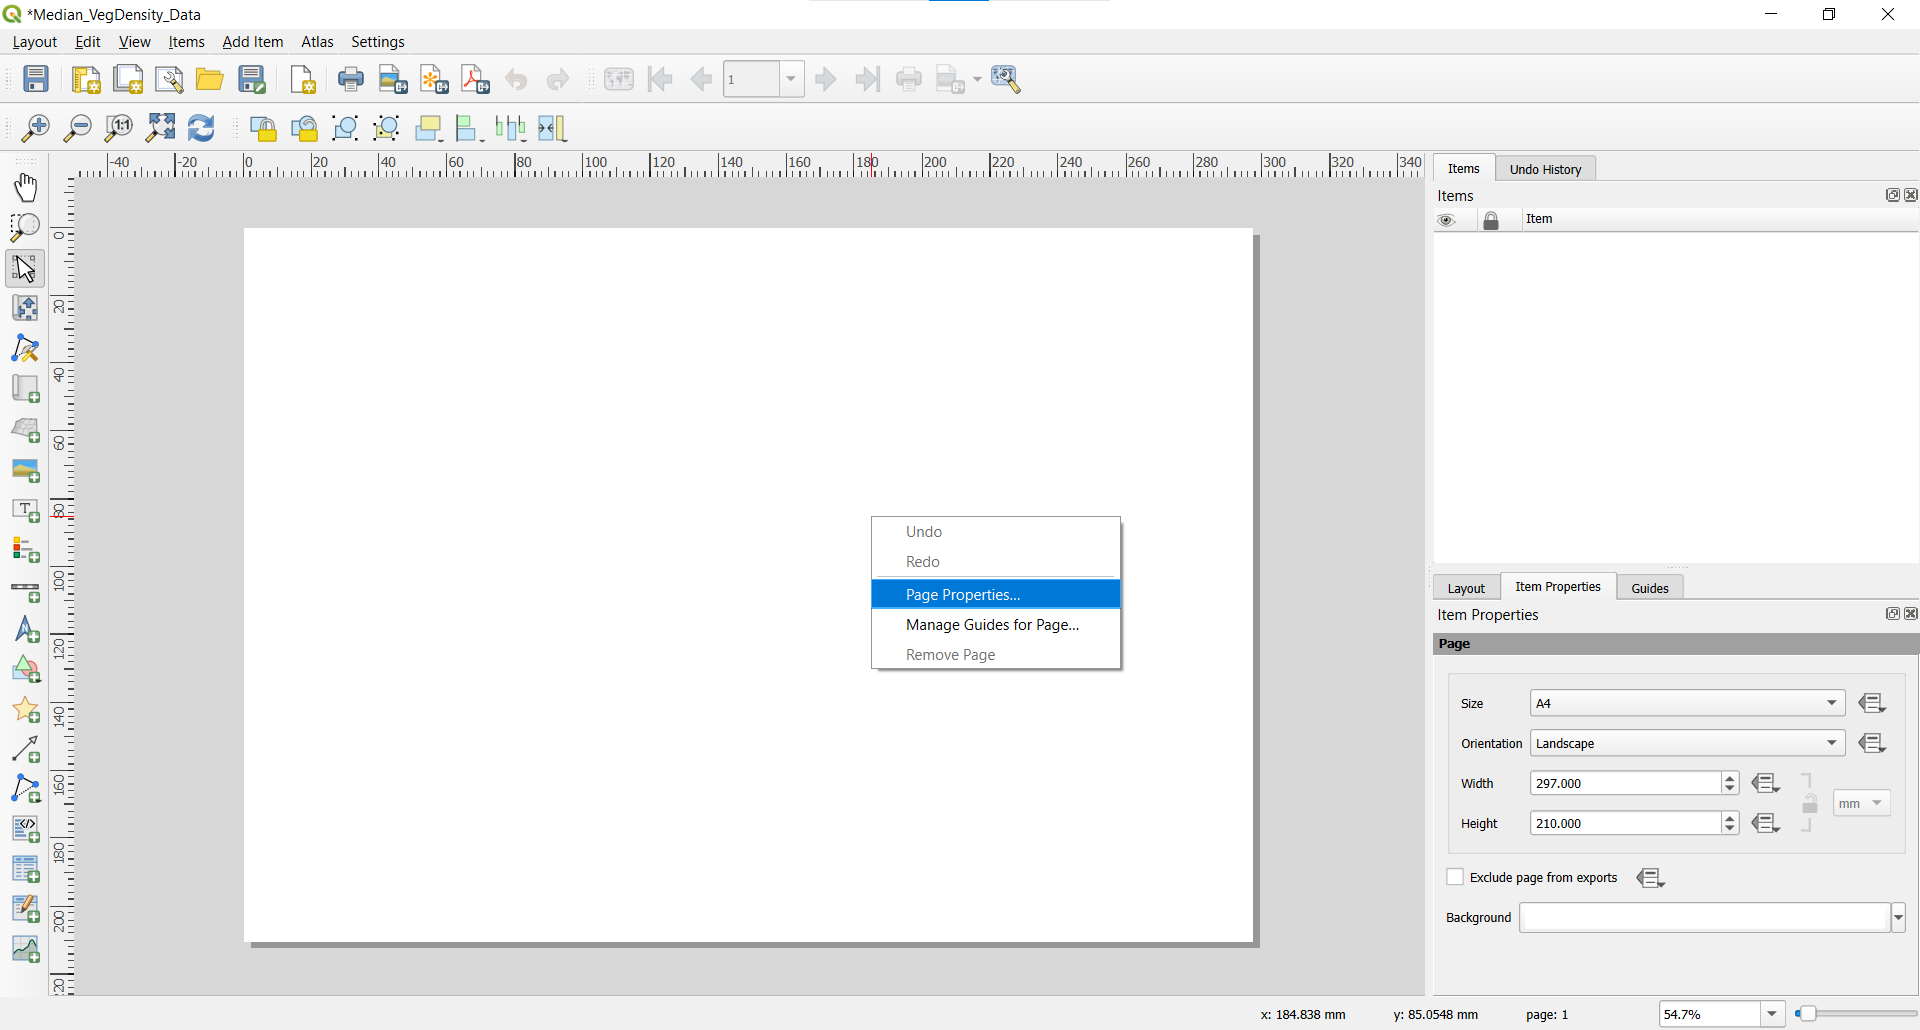
\includegraphics{./images/LayoutWindow.png}

}

\caption{Example of a blank layout, with Page Properties pane open}

\end{figure}

The default size is A4, or an 8.5x11 piece of paper; I often find myself
using a custom sized, square sheet for NYC maps, so I change the
``Size'' to ``Custom'', change the units from millimeters to inches, and
specify the width and height as 7 inches.

This is basically the blank area with which we can fill with a map (or
maps!) - to enable bringing a map from the main QGIS window into a Print
Layout start by clicking
\includesvg{index_files/mediabag/mActionAddMap.svg}, then click and drag
across the page area. Whatever you had in the main QGIS window should
now appear. Also, the ``Item properties'' should be tied to the map that
you just drew, with parameters associated with that (e.g., showing the
map scale, any desired rotation, among many other things). At the top of
the item properties for the Map, you will see icons, which will, for
example, refresh what is shown on the page to reflect what is in the
main map canvas, if you have changed things there. So, go back to your
map canvas and adjust things to start working towards what you might
like to show in a map!

\textbf{\emph{Once you have a set of layers and styles you generally
like for your map, in the Item Properties for the Map, check the ``Lock
Layers'' box, which will not affect the main map canvas, but will keep
what is shown in the Print Layout as they are. Otherwise, any changes
you make in the main map canvas would show up here.}}

\begin{figure}

{\centering 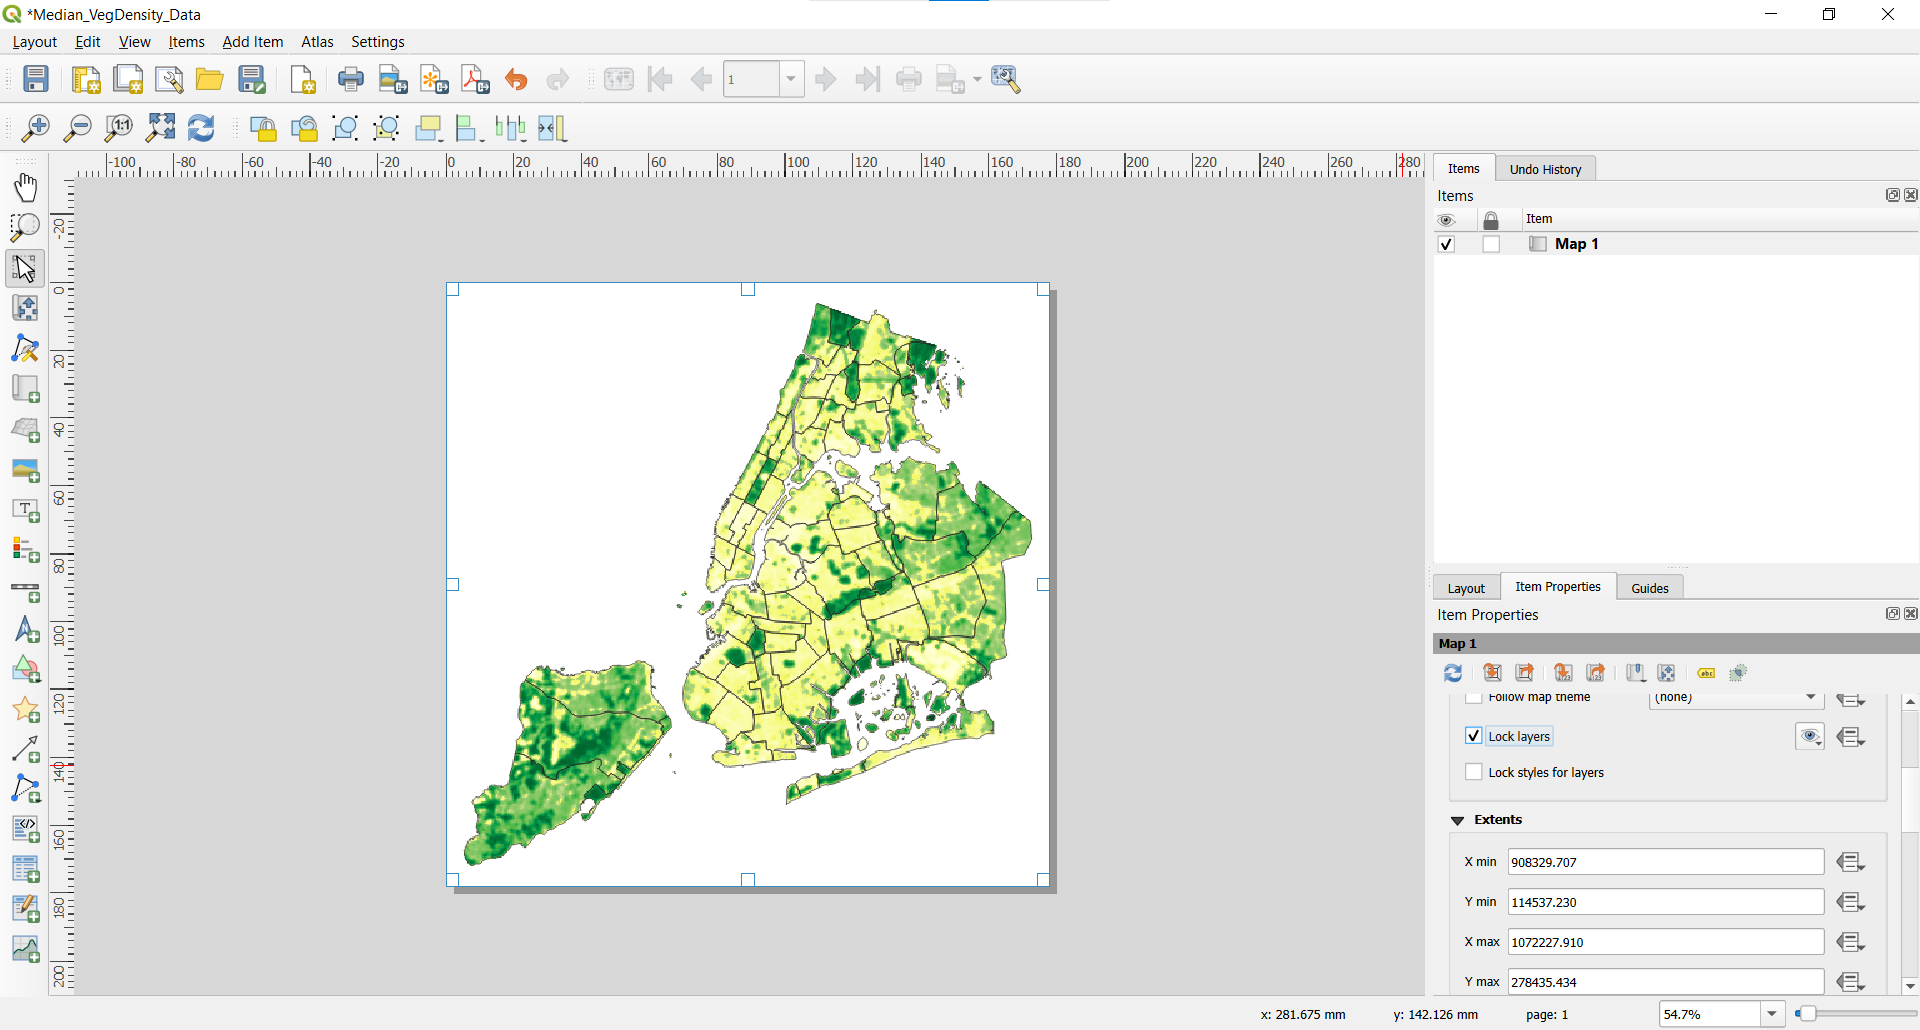
\includegraphics{./images/PrintLayout_DesiredLayers.png}

}

\caption{The start of a map with Community District Boundaries and the
Vegetation Density layer}

\end{figure}

Now, you can start adding things that might help make the map make sense
- browse around and find things that you can add (e.g.,
\includesvg{index_files/mediabag/mActionAddLegend.svg} for a legend,
\includesvg{index_files/mediabag/north_arrow.svg} for a North arrow).

With all of these things you can add, just as you did to add the map to
the layout, you will click the respective icon, then click and drag to
lay out a box of where the item should be placed. For each item, there
will be a separate different options for the ``Item Properties.''

Legends can be tricky, as by default all layers are included. However,
you can check the box in the Item Properties for the legend, in the area
with ``Legend Items,'' to only show the items within the map being
shown. You'll see the legend entries on the map decrease to only the
layers being shown. Additionally, there are lots of options for fonts,
spacing, and other aspects, worth browsing around for. Further, for each
legend entry, you can, in the Item Properties, click the text to edit
what the text will be in the legend. In my experience it can be helpful,
for individual maps, to turn off ``Auto Update'' as you may edit things
like labels for the legend items, and do not want those edits to be lost
as QGIS updates based on what is being done through the main window
(e.g., based on editing layer names or similar).

By default, with a raster, the legend will say something like ``Band 1
(Gray),'' as with the Vegetation Density data. In the Legend Items list,
you can expand the legend entries for that layer, select that row of
information that says ``Band 1 (Gray'') and then click
\includesvg{index_files/mediabag/symbologyRemove.svg} below to remove
it. (The box for Auto-Update must be unchecked to do this.)

And note, there are different ways to improve the appearance of legends,
such as for rasters, in the symbology settings for the layers - what is
shown below is just the basic example to start with.

\begin{figure}

{\centering 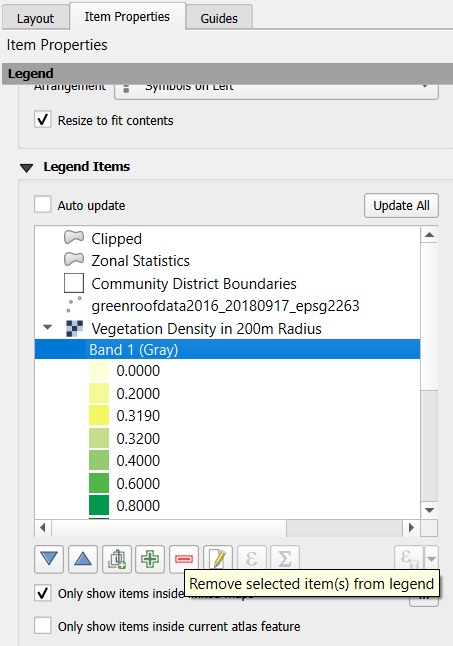
\includegraphics{./images/legend_edit.png}

}

\caption{Using the Item Properties tab to adjust the legend entries}

\end{figure}

While you can add a new text box in the layout for a map title, I've
decided to use the Legend Title space as a place for the map title. For
the full title I wanted to include, ``Vegetation Density Across NYC
Community Districts'' would overlap portions of the data being shown, I
used the ability to specify a character on which to wrap the text - I
used a backslash but you could chose any character that is not part of
the title. (In the text of the title, below, you can see I inserted a
backslash between ``NYC'' and ``Community'' and specified that as the
``wrap text on'' character, and the backslash is not visible in the
title on the page).

\begin{figure}

{\centering 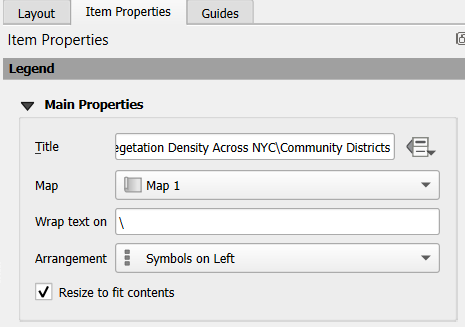
\includegraphics{./images/LegendTitle.png}

}

\caption{Using the ``Wrap text on'' functionality for legend title
adjustments}

\end{figure}

I also scrolled down in the Item Properties for the legend, and
unchecked the ``Background'' so that if the legend box overlapped with
parts of the map itself, it was not visible.

As an example, below is the map I produced.

\begin{figure}

{\centering 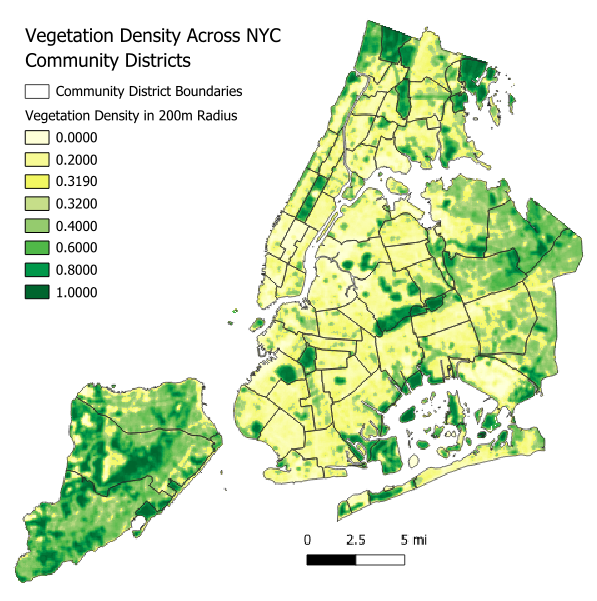
\includegraphics{./images/final_map.png}

}

\caption{Sample map from QGIS}

\end{figure}

You can then export the map to various formats including as images
(\includesvg{index_files/mediabag/mActionSaveMapAsImag.svg}), PDFs
(\includesvg{index_files/mediabag/mActionSaveAsPDF.svg}), and SVG files
(\includesvg{index_files/mediabag/mActionSaveAsSVG.svg})



\end{document}
